\documentclass[a4paper, 14pt]{article}
\usepackage[pdftex,
    pdfauthor={Егоров Геннадий Викторович},
    pdftitle={Сбоник лекций по курсу радиационнной физики для 4 курса Медицинской физики},
    pdfsubject={Радиационная физика},
    pdfkeywords={ ИИ, Дозиметрия, Радиоактивность, 4 курс Медицинская физика},
    pdfproducer={LuaLatex with hyperref},
    pdfcreator={Lualatex},
    hidelinks
]{hyperref}
\usepackage{latexsym,amsmath,amssymb,amsbsy,graphicx}
\usepackage[font=small,labelfont=it]{caption}
\usepackage{tikz}
\usepackage{placeins}
\usepackage{pgfplots}
\usepackage{wrapfig}
\usepackage{tablefootnote}
\usepackage{icomma}
\usepackage[version=4]{mhchem} % the canonical chemistry package(example: \ce{^{32}_{15}P})
\usepackage{multirow}
\usepackage{hhline} %Чёрточки в таблицах
\usepackage{array}
\newcolumntype{C}[1]{>{\centering\arraybackslash}p{#1}}
\graphicspath{{images/}}
\DeclareGraphicsExtensions{.pdf,.png,.jpg}
%%%%%% Для красивого отображения рисунков из inkscape
% \usepackage{import}
% \usepackage{xifthen}
% \usepackage{pdfpages}
% \usepackage{transparent}
% \newcommand{\incfig}[1]{%
%     \def\svgwidth{\columnwidth}
%     \import{./images/}{#1.pdf_tex}
% }
%%%%%%%%%%%%
% \usepackage[dvipsnames]{xcolor} % dvipsnames добавляет 68 цветов https://ru.overleaf.com/learn/latex/Using_colours_in_LaTeX
\renewcommand{\emph}[1]{{\color{orange}{\textit{\textbf{#1}}}}}
%%%%%%%%%%%%%%%%%%%%%%%%Оформление по ГОСТу
\usepackage{fontspec}
\setmainfont[Renderer=Basic,Ligatures={TeX}]{Times New Roman}
\usepackage[english, russian]{babel} %Поддержка русского языка
\usepackage[14pt]{extsizes} % для того чтобы задать нестандартный 14-ый размер шрифта
\usepackage{indentfirst} %Задаёт отступ самого первого абзаца
\setlength\parindent{1.25cm}
\usepackage[a4paper, left=3cm, top=1.5cm, right=1.5cm, bottom=2cm]{geometry}
\usepackage{setspace}
\sloppy %Выравнивание текст по ширине
\onehalfspacing %Полуторный интервал
\title{Лекции по радиационной физике}
\author{\href{mailto:gennadyegorow@yandex.ru}{Егоров Г.В.} \and \href{mailto:www-kirill.pilipenko@yandex.ru}{Пилипенко К.С.}}
\date{\selectlanguage{russian}\today}
\begin{document}
\maketitle
\tableofcontents
\section{Предмет и метод радиационной биофизики. Актуальность исследования
биологического действия ионизирующего излучения. Разделы радиобиологии}
\emph{Радиационная биофизика}~---~это наука, изучающая молекулярные механизмы
биологического действия ионизирующего и неионизирующего излучения на органы,
вычисляющие последовательную картину изменений, начиная от поглощенной
энергии радиации отдельных молекул до сложных биологических изменений в клетке
и органе.

Радиационная биофизика изучает радиобиологические проблемы с позиции
биофизики. Если радиобиология изучает влияние излучения на биологические
объекты, то биофизика изучает молекулярные взаимодействия, лежащие в основе
нормальных и патологических жизненных явлений.

\emph{Ионизирующим излучением} (проникающей радиацией, ИИ) называют
высокочастотные электромагнитные излучения энергетических фотонов, которые
превышает величину потенциала ионизации больше, чем 10 эВ. К ИИ относятся рентгеновское излучение и гамма-излучение.

\noindent 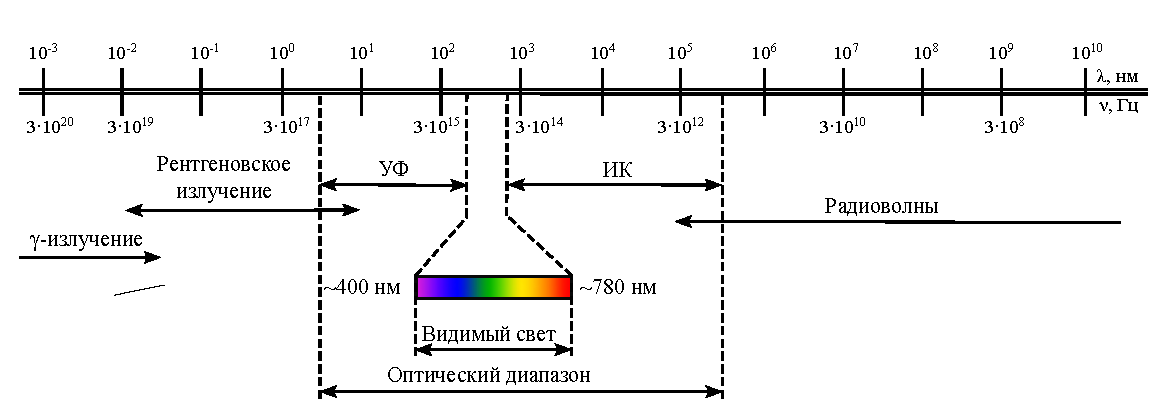
\includegraphics[width=\textwidth]{EMW.pdf}

\[ E = h\nu = \frac{hc}{\gamma}, 1\;\text{эВ} = 1,6 \cdot 10^{-19}\;\text{Дж}\]
\[ E = 10\;\text{эВ} = 1,6 \cdot 10^{-18}\;\text{Дж}\]
\[ \gamma = \frac{hc}{E} = \frac{6,6\cdot 10^{-34} \cdot 3 \cdot 10^8}{1,6 \cdot 10^{-19}} = 1,2 \cdot 10^{-7}\;\text{м} = 120\;\text{нм}\]
Рентгеновское излучение и гамма-излучение отличаются по энергии, длине
волны и по происхождению.

Рентгеновское излучение делится на \textit{тормозное} и \textit{характеристическое}.

\emph{Тормозное} возникает при торможении заряженных частиц при большом
ускорении. Энергетический спектр является непрерывным.

\emph{Характеристическое} возникает при переходах между далеко расположенными
энергетическими уровнями. Спектр излучения дискретный.

Гамма-излучение возникает либо при ядерных реакциях, либо при переходах в
энергетических уровнях в ядрах.

\emph{Оптические излучения} не способны к ионизации молекул, лишены высокой
проникающей способности.
К ИИ также относятся: корпускулярные излучения, а именно: $\beta$-частицы, т.е. электроны, позитроны, протоны, $\alpha$-частицы, так же нейтроны и др. частицы.

Актуальность исследования биологического действия ИИ:
\begin{enumerate}
    \item Все живое постоянно подвергается воздействию постоянного естественного
    радиационного фона;
    \begin{itemize}
        \item космическая радиация;
        \item излучение радиоактивных элементов, залегающих в поверхностных слоях
        земной коры и входящих в состав живых организмов и продуктов питания;
    \end{itemize}
    \item В связи с техногенной деятельностью человека (взрывы, аварии)
    радиационный фон во многих регионах значительно выше естественного, поэтому
    возникает необходимость исследования влияния этого повышенного фона на здоровье
    и жизнь человека;
    \item  ИИ используется как диагностическое и
    терапевтическое средство при многочисленных заболеваниях
\end{enumerate}
Радиационная терапия основана на изучении механизмов взаимодействия
излучения с веществом.

\emph{Радиобиология}~--~это комплексная наука, в которой развиваются многие
направления:
\begin{enumerate}
    \item Радиационная экология и генетика
    \item Радиационная биохимия и цитология
    \item Радиационная медицина и генетика
    \item Радиационная биофизика
\end{enumerate}

\emph{Радиационная биофизика} занимает особое место в радиобиологии. Она
выясняет физико-химические и молекулярные механизмы первичных процессов
лучевых изменений, протекающих с момента возникновения ионизирующего
возбуждения атомов и молекул до появления видимых структурных и функциональных изменений.

Для решения этой задачи необходимо углубленный анализ процессов,
проходимых после поглощения энергии квантов в живой системе, описание всех
этапов в терминах молекулярных изменений и создание единой картины, отражающей
всю последовательность реакций, приводящих в зависимости величины дозы к
лучевым изменениям или поражениям.

\section{История развития радиационной биофизики}
Радиобиология возникла после открытия рентгеновского излучения, которое
произошло в конце 19 веке.

В декабре 1895г., Рентгеном был сделан первый рентгеновский снимок кисти своей руки. Результаты работы были изложены в рукописи об открытии катодных проникающих Х-лучей.

В январе 1896 г. брошюра Рентгена «Новый род лучей» вышла в свет на
нескольких языках, открытие стало достоянием мировой общественности.

Март 1996, Анри Беккерель обнаружил явление~---~самопроизвольное испускание
невидимых глазу проникающих излучений ($\alpha, \beta$ и $\gamma$), исходящих от солей урана.

Через два года Мария и Пьер Кюри выделили из урановой смолы ранее не
известные элементы, так же, подобно урану, испускающие излучения, которым они
дали название радий и полоний. Для явления, свойственного этим, а в последующем
другим подобным элементам был предложен термин \emph{радиоактивность}.

Открытие урановых, а затем и ториевых лучей послужило началом
исследований \textit{естественной (природной) радиоактивности}.

1934г. Ирен Кюри и Фридерих Жулио Кюри открыли новое явление~---~искусственную радиоактивность (при исследовании ядерной реакции $^{27}Аl(\alpha,n)^{30}P$ %TODO: Нужно уточнить реакцию
обнаружили образование нового, не встречающегося ранее в природе радионуклида~---~фосфора \ce{^{30}P}).

\subsection{Развитие радиобиологии}
Петербуржский физиолог Тарханов провел исследование на лягушках и
насекомых и пришел к выводу, что Х-лучами можно не только фотографировать, но и
влиять на ход жизненных функций.

Ефим Лондон в 1896 году начал исследование по экспериментальной
радиобиологии.

Первая официальная информация о патологическом влиянии радиации была
опубликована в 1901 году, которая сообщила, что радий вызывает ожоги кожи.

\emph{Важными задачами} радиобиологии в то время была необходимость точной и
количественной оценки дозы радиации, вначале появились условные единицы
биологических доз.

% HED (кожная-эритемная доза) %TODO: Зачем это здесь?
В 1901 и последующие годы появилось множество работ о лучевом поражении
кожи. В 1902 году описан первый случай лучевого рака кожи. Выяснилось, что
возникающая радиация не только воздействует на кожу, но и вызывает лучевое
поражение внутренних органов и тканей, а также гибель живых организмов и
человека. Опыты Лондона в России и Хейкеля в Германии.

В Последующие годы выяснились сведения о высокой биологической эффективности нового вида излучений стимулировало мощный взрыв радиобиологических работ, характеризующий \emph{начальный, описательный период} в истории радиобиологии.  

\subsection{Открытие закона радиочувствительности клеток}
В 1906 г. французские радиобиологи Жан Бергонье и Луи Трибондо сформулировали фундаментальный \emph{закон (правило) радиочувствительности клеток:} \textit{ ИИ оказывает тем большее повреждающее действие на клетки, чем интенсивнее те делятся и чем менее определенно выражены их морфология и функция, т. е. чем менее они дифференцированны}. 

По мере накопления фактов становилось ясным, что ИИ, в зависимости от интенсивности источника радиации и длительности облучения, способны вызывать повреждения и гибель любого биологического объекта, любой биологической системы.

Начиная с 1910 г. М. И. Неменов и сотрудники публикуют работы по
выяснению изменений обмена веществ при лучевом поражении и о сходстве лучевых
изменений с процессами патологии раннего старения.

Первая в мире монография (Е. С. Лондон <<Радий в биологии и медицине>>)
вышла в свет в 1911 г. на немецком языке, а в 1968 г. переведена на русский язык в
издательстве \textit{<<Медицина>>}.

В 1918 г. в Петербурге был открыт первый в стране радиобиологический
Государственный институт рентгенологии и радиологии, организатором
и директором стал рентгенолог М. И. Неменов.

В 1925 г. была наглядно показана важная роль биохимических процессов в
развитии лучевого поражения. Анцель и Винтенбергер в опытах на куриных
эмбрионах обнаружили, что интенсивность обменных процессов оказывается
основополагающей в формировании проявлений лучевого поражения. Это
наблюдение позволило авторам предсказать участие трех существенных моментов в
развитии лучевого поражения:
\begin{itemize}
    \item \textit{наличие первичного радиационного повреждения;}
    \item \textit{существование факторов, способствующих усилению этого повреждения;}
    \item \textit{влияние восстанавливающих факторов.}
\end{itemize}

Постепенно формировалось представление, согласно которому степень лучевого
поражения определяется не только интенсивностью первичного
повреждения, но и физиологическим состоянием организма и характером
метаболических процессов в нем. Для возникновения острой лучевой болезни
должен произойти сложный комплекс взаимосвязанных изменений в организме,
появление которых зависит от величины дозы, характера и способа облучения, от
времени, прошедшего после лучевого воздействия и биологической особенности
организма (его радиочувствительности).

Исследование динамики и механизмов формирования биохимических нарушений при лучевых поражениях заняло все дальнейшие годы развития радиобиологии и позволило собрать ценнейший материал для характеристики и классификации клинических проявлений радиационного эффекта. Это привело исследователей к установлению количественных принципов, связывающих радиобиологические эффекты с дозой облучения. 

\subsection{Появление количественной радиобиологии}
В 20-е годы XX в. был открыт следующий, \emph{второй период в развитии радиобиологии~---~период изучения механизмов действия ИИ на биологические объекты и системы} и положено начало формированию \emph{количественной радиобиологии}. Начались интенсивные поиски критических биологических молекулярных и клеточных структур, а также органов и тканей облучаемых организмов, ответственных за развитие лучевого поражения, ведущего к смертельному исходу.

\emph{Открытие радиобиологического парадокса:} энергия ИИ несопоставима мала по сравнению с тем эффектом, который она вызывает (в тепловом измерении). 

В 1925-1927 гг. советскими учеными Г.А.Надсоном и Г. С. Филипповым обнружили в экспериментах на дрожжевых клетках, а позднее Г. Мёллером (США) на дрозофиле \emph{эффекта радиационного мутагенеза}, проявляющегося не только в повреждении \textit{«вещества наследственности»}, но и в образовании стойких необратимых изменений в нем, передающихся по наследству. Были получены строгие доказательства возникновения мутаций под влиянием облучения. 

С открытием мутагенного действия излучений многие радиобиологи перешли к изучению \emph{ единичной реакции дискретных биологических структур (генов, хромосом) на радиационное воздействие}. В это же время значительно совершенствуются методы дозиметрии излучений, вводится ионизационная единица дозы~---~рентген. 

Появляется возможность количественного анализа биологического действия излучений, основанного на выяснении зависимости между наблюдаемым биологическим эффектом и дозой радиации, поглощенной изучаемой системой. Такие эксперименты проводились не только на ядерных наследственных структурах, но и на колониях клеток, вирусных частицах, препаратах ферментов. Результаты, полученные в точных количественных опытах, свидетельствовали о вероятностном характере проявления единичной реакции объекта в ответ на облучение в данной дозе радиации. 
% Иначе говоря, при облучении однородных объектов (клетки одной линии, молекулы одного типа и т.д.) наблюдали, что при любой малой дозе радиации некоторое число объектов оказывается пораженным, а другие сохраняют исходные свойства; \emph{при самой большой дозе радиации небольшая доля объектов все еще остается непораженной. Кривые «доза-эффект» в этих случаях имели
% экспоненциальный характер} и их можно было надежно экстраполировать к нулевой
% точке.

Обнаруженный эффект нельзя было объяснить естественной вариабельностью:
речь шла о генетически однородных клетках и вирусных частицах или молекулах
одного типа. Его трактовка потребовала прежде всего, представлений о
вероятностном характере поглощения энергии излучений, о дискретной природе
частиц, составляющих  ИИ, о физически микрогетерогенной
организации биологических структур.

Начало исследований в области количественной радиобиологии (20-е гг.) и
стало рождением радиационной биофизики, так как впервые для объяснения
радиобиологических феноменов и создания общей теории биологического действия
 ИИ в качестве отправных концепций потребовалось
использовать теоретические положения квантовой механики и ядерной физики.

В 1922 г. Ф. Дессауэр, предложил \emph{теорию «точечного нагрева»}.
 ИИ обладают малой объемной плотностью, однако отдельные
фотоны несут гигантский запас энергии. Ф. Дессауэр предположил, что при
поглощении системой относительно небольшой общей энергии (смертельная для
человека доза облучения вызывает нагрев тела всего на 0,001$^\circ$С) некоторые
дискретные микрообъемы поглощают настолько большие порции энергии, что
действие  ИИ можно сравнить с таким микролокальным
нагревом, который вызывает глубокие структурные изменения и в конечном счете
биологическое поражение. Вероятностный характер проявления эффекта у
отдельных объектов автор гипотезы объяснял статистическим распределением
\textit{«точечного тепла»}. Так впервые \emph{физический принцип попадания был использован
в исследованиях количественной радиобиологии}.

Дальнейшее его развитие связано с работами Дж. Кроутера, Д. Ли, К. Г. Циммера, Н. В. Тимофеева-Ресовского, В. И. Корогодина и др. 

Работы этого периода оказали большое влияние на дальнейшее развитие радиационной биофизики, превратили ее в одну из самых точных биологических дисциплин. Математический аппарат, развитый в этих работах, позволил с достаточной надежностью судить о \textit{«пусковых событиях»}, приводящих к регистрируемым в эксперименте биологическим реакциям (мутации, гибель клетки и др.) и оценивать параметры «мишени», ответственной за наблюдаемый радиобиологический эффект.
% Согласно \emph{принципу попадания}, начальный физический пусковой механизм, необходимый для возникновения конечной биологической реакции, обусловлен случайным взаимодействием ионизирующего излучения с веществом. В силу этого в каждую молекулу или клетку происходит неодинаковое число попаданий. С принципом попаданий тесно связана \emph{теория мишени}, основанная на принципе гетерогенности строения живых систем, поражение излучением отдельных элементов которых имеет не одинаковое значение для данной системы. Например, необратимое повреждение уникальной клеточной структуры фатально для клетки, тогда как такое же повреждение иных, множественных структур для судьбы клетки может иметь существенно меньшее значение. 
В многочисленных работах получены новые факты высокой радиочувствительности делящихся клеток, клеточного ядра, молекулы ДНК. 

Сейчас хорошо известно, что \emph{высокой радиочувствительностью обладают делящиеся клетки, клеточное ядро и молекула ДНК}, причём нарушения генетических структур могут проявляться как сразу после облучения, так и отдаленно, в потомках, даже спустя несколько поколений, становясь в организме причиной возникновения злокачественных опухолей, а также различных уродств развития. 
%TODO:
% Обнаруженный эффект можно объяснить, используя представления о вероятностном характере поглощения энергии излучений и о дискретной природе частиц, составляющих  ИИ. 

Выяснилось, что даже при облучении в малых дозах происходит много тысяч актов ионизации молекул, но лишь некоторые из образовавшихся нарушений структуры и функции клеток приводят клетку к потере способности деления и гибели. 

\emph{Критической мишенью клетки является молекула ДНК.} Применение теории мишени ограничено. Конкретная ответная реакция на облучение зависит не только от попадания ДНК, но и от ряда свойств самого биологического объекта, например, от способности устранять повреждения - системный ответ клетки на облучение. 

Системный ответ носит \textit{статистический характер}. Важным направлением в статистической физике является создание математической модели, которая является формализованным выражением теоретических закономерностей. Усовершенствование моделей связано с повышением доступности и быстродействием компьютеров. 

% \subsection{Появление радиационной биофизики}
Радиационная биофизика зародилась в 20 г. ХХ в., когда впервые для объяснения радиобиологических явлений стали использовать теоретические положения квантовой механики и ядерной физики. 

Согласно \emph{принципу попадания} начальный физический пусковой механизм, необходимый для возникновения биологической реакции обусловлен случайным взаимодействием ИИ с веществом. 

С принципом попадания связана \emph{теория мишени}, основанная на принципе гетерогенности. Необратимое повреждение уникальной клеточной структуры фатально для клетки, тогда как такое же повреждение других структур имеет меньшее значение. 

В середине ХХ столетия после бомбардировок Хиросимы и Нагасаки начался \emph{3 этап в развитии радиобиологии}. Происходит перенос акцентов в развитии радиологии и радиационной биофизики. Развиваются исследования молекулярных механизмов действия излучения. Этому способствовал ряд достижений в области биофизики и молекулярной биологии, а именно доказательство биологической роли ДНК и расшифровка ее структуры. 

В 40-е гг. было обнаружено зарождение в облучаемом растворе высокоактивных продуктов \emph{радиолиза воды}~---~свободных радикалов, способных диффундировать на значительные расстояния и поражать биологические структуры. 

Радиационная биофизика начинает оперировать представлениями о \emph{«непрямом действии»} излучения, опосредованном активными продуктами радиолиза воды. 

Были изучены физико-химические свойства первичных продуктов радиолиза воды и характер их взаимодействия с макромолекулами клетки. Это дало возможность приступить к исследованиям средств защиты (\emph{радиопротекторов}) от действия  ИИ. 

В 1942 г. В. Дейлу удается снизить поражающее действие радиации на ферменты введением в раствор ряда веществ~---~перехватчиков радикалов. 

В 1949 была доказана способность ряда веществ защищать млекопитающих от лучевого поражения. В опытах Х. Патта с соавторами введение цистеина за 10 мин до облучения защищало крыс от неминуемой гибели. 

В мире начинается интенсивный поиск эффективных радиозащитных препаратов. Формируется самостоятельное направление радиационной биофизики~---~выяснение механизмов модифицированной радиочувствительности биологических объектов. 

Было установлено, что важную роль в радиозащитных препаратах играет понижение содержания кислорода в тканях. 

В середине 60-х гг. З. Бак и П. Александер сформулировали \emph{гипотезу «биохимического шока»}, согласно которой различные радиопротекторы однотипно изменяют метаболические процессы, переводя клетки в состояние повышенной устойчивости к действию ионизирующей радиации. 

В дальнейшем появился ряд исследований, посвященных анализу конкретных биохимических изменений, возникающих под влиянием радиозащитных агентов и модифицирующих радиорезистентность организма. Возникли гипотезы «комплексного биохимического механизма действия радиозащитных средств», «сульфгидрильная гипотеза». 

Исследования привели к накоплению обширного фактического материала по общей картине лучевого поражения и его модификации, они позволили наметить пути к выявлению основных закономерностей зарождения пусковых физико-химических процессов, механизмов ослабления или усиления первичных лучевых реакций. В результате на первый план вышли исследования, посвященные анализу физико- химических процессов, протекающих в клетке от момента возникновения начальных структурных повреждений до проявления выраженных биохимических и морфологических изменений. 

Анализируется модифицирующее действие кислорода, температуры и других агентов, влияющих на развитие лучевого поражения биологических объектов. 

Авария на Чернобыльской АЭС в 1986 г., снятие секретов с информации о ее последствиях, последствиях других радиационных аварий и ядерных испытаний открыли новый, \emph{четвертый период в истории радиобиологических исследований}.

Для решения проблем, возникших после Чернобыльской катастрофы, накопленные знания и имеющийся опыт традиционной радиобиологии н медицины оказываются явно недостаточными, и поэтому в современной радиобиологии стали быстро развиваться новые направления: 

\begin{itemize}
    \item изучение биологического действия излучений в малых дозах и отдаленных последствий облучения; 
    \item исследование комбинированного действия широкого спектра радионуклидов с химическими загрязнителями среды; 
    \item поиск принципиально новых средств защиты от хронического облучения. 
\end{itemize}

Перед радиационной биофизикой возникли новые задачи. Наиболее важными оказались фундаментальные исследования механизмов радиобиологических эффектов, вызываемых слабыми воздействиями, поскольку оказалось, что эффекты, вызываемые  ИИ в малых дозах, нельзя оценивать путем простой экстраполяции в область малых доз данных, полученных при больших дозах. 

Открылись \emph{принципиально новые явления при изучении эффектов малых доз}. Это и повышенная чувствительность биообъектов к воздействию радиации в сверхмалых дозах, переходящая к повышенной радиорезистентности~---~\emph{адаптивному ответу}~---~при более высоких нелетальных дозах. Это и \textit{стимулирующее действие излучений на рост, развитие и другие физиологические показатели} (эффект гормезиса), а также \textit{необычное снижение выраженности радиобиологических эффектов по мере увеличения мощности малой дозы} (\emph{обратный эффект мощностей доз}). 

Кривая зависимости \emph{доза-эффект} в области малых доз синусоидальная. 

Большое значение приобретают исследования механизмов регуляции, происходящих в биоматериале (БМ) и ДНК и образующихся в них под действием  ИИ оксирадикалов и других продуктов окисления. 

На рубеже столетий было открыто важное явление: \textit{способность облученной клетки передавать путем контактов или секреции сигналы, действующие на соседние необлученные клетки подобно облучению}~---~\emph{эффект свидетеля}. 

Современный период диктует новые переходы к разработке методов химической защиты. Появилась необходимость в исследованиях пищевых продуктов и препаратов, способных, не оказывая вредного побочного действия на организм снижать или предотвращать хроническое низкоинтенсивное облучение. Большое внимание уделяется средствам, выводящим радионуклиды из организма.

\section{Виды и характеристики ионизирующих излучений}
К ионизирующим излучениям относят: фотоны электромагнитного излучения ($\lambda < 20$ нм) и корпускулярное излучение, т.е. ускоренные частицы и ядра электронов.

Фотонное излучение делится на: рентгеновское (от ~10 эВ до 500 кэВ) и $\gamma$-{\nolinebreak}излучение (более 100 кэВ). Диапазоны энергии этих двух видов излучения перекрываются, но отличаются по происхождению.

\subsection{Рентгеновское излучение}
\emph{Рентгеновское излучение}~---~это коротковолновое ЭМ излучение, с диапазоном длины волны от 25~нм до $2,5\cdot 10^{-3}$~нм, которое возникает двумя путями:
\begin{enumerate}
    \item \emph{характеристическое} рентгеновское излучение~---~при переходах между
    далеко расположенными энергетическими уровнями;
    \item \emph{тормозное} рентгеновское излучение возникает при торможении частиц
    высоких энергий в кулоновском поле ядер атомов вещества поглотителя (кинескоп).
\end{enumerate}

\emph{Тормозное} излучение представляет собой излучение со \emph{сплошным} спектром, в то время как спектр \emph{характеристического} рентгеновского излучения является \emph{дискретным}. Также рентгеновское излучения по энергии фотона делят на:
\begin{itemize}
    \item $E_\text{ф}<$ 50 кэВ~---~мягкое ($\lambda > 25$ нм);
    \item $E_\text{ф}>$ 50 кэВ~---~жесткое ($\lambda < 25$ нм).
\end{itemize}

При возникновении тормозного излучения электроны, испытывающие торможение в состоянии с законами электродинамики, излучают ЭМГ-волны в зависимости от величины ускорения частицы. При энергии электрона выше 20 МэВ потеря энергии на излучение становится почти пропорциональной самой энергии: 
\begin{equation}
    \left ( - \frac{dE}{dt} \right ) \sim Z^2 (E_k + m_0c^2)\cdot N,
\end{equation}
где $E_k$~---~кинетическая энергия электрона, Z~---~заряд ядра материала поглотителя, N~---~число атомов в 1 см$^3$ поглотителя. Из этого соотношения следует, что энергия квантов рентгеновского излучения пропорциональна поглощенной энергии и находится в квадратной зависимости от атомного номера вещества поглотителя. 

Это учитывается при конструировании рентгеновских трубок (рис. \ref{x-rayTube}), в которых электроны преображают высокую энергию при ускорении в электрическом поле, создаваемом за счет высокого напряжения между катодом и анодом. 
\begin{figure}[htbp]
    \centering
    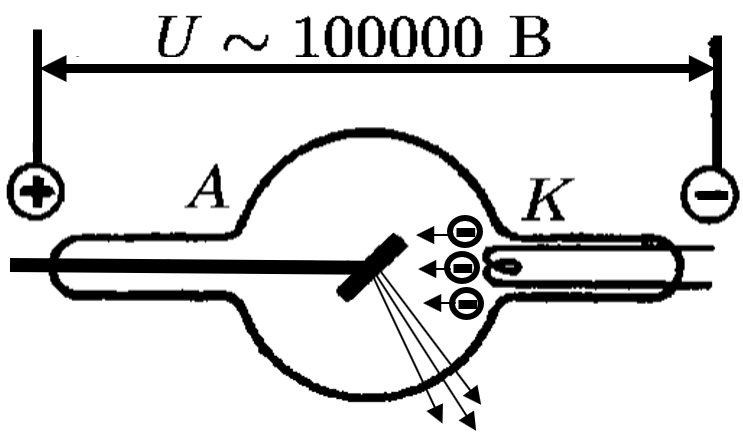
\includegraphics[width=.5\textwidth]{x-rayTube.png}
    \caption{Схема рентгеновской трубки}
    \label{x-rayTube}
\end{figure}

Анод изготавливается из материалов с большим атомным номером. В кулоновском поле в атомах анода происходит термоэлектронное ускорение электронов, при этом возникает рентгеновское излучение. При бомбардировке анода электронами, только 0,2\% их кинетической энергии испускаются в виде квантового рентгеновского излучения, а остальная энергия рассеивается в виде тепла. Поэтому необходимо надежное охлаждение рентгеновских трубок. 

\subsection{γ-излучение}
\emph{γ-излучение}~---~ЭМ излучение с малой длиной волны (λ<0,1 нм) и энергией от 50 кэВ до 10 МэВ, которое возникает:
\begin{itemize}
    \item при ядерных реакциях и распаде элементарных частиц;
    \item либо при аннигиляции пар частиц.
\end{itemize} 

\emph{Аннигиляция}~---~взаимное уничтожение элементарных частиц с образованием γ-излучения. Например, аннигиляция электрона и позитрона. 

В биологических исследованиях в качестве источника γ-излучения используют радиоактивный изотоп кобальта \ce{_{27}^{60}Co}. Такой источник кобальтового излучения называется \emph{кобальтовой пушкой}.

γ-кванты генерируются в процессе радиоактивного распада \ce{_{27}^{60}Co} и \ce{_{28}^{60}Ni}. Возбужденное ядро Ni переходит в стабильное состояние с последующим испусканием γ-квантов с энергией $Е_1=1,17$ МэВ; $Е_2=1,33$ МэВ.

\subsection{Корпускулярное излучение}
\emph{К корпускулярному излучению} относят электроны, позитроны, нейтроны, $\alpha$-частицы, протоны, ускоренные ионы, ядерные фрагменты и осколки деления ядер, а также многие нестабильные частицы. 

\emph{К электронному} излучению относят $\beta$-частицы (электроны с энергией 0,002~--~2,3 МэВ, возникающие при распаде радиоактивных ядер) и ускоренные электроны, которые создаются ускорителями электронов (с энергией от кэВ до сотен МэВ). 

Ядра атома гелия называются $\alpha$-частицами, когда они образуются при распаде некоторых радионуклидов и несут энергию до $\sim$10 МэВ. Те же ядра, ионизированные и ускоренные, образуют пучки ионов гелия. Эти и другие пучки заряженных частиц~---~протонов, дейтронов и вообще любых многозарядных тяжелых ионов (например, углерода)~---~получают в протонных и ионных ускорителях. На них при облучении мишеней получают также пучки нейтральных частиц~---~фотонов и нейтронов, и даже пучки радиоактивных ионов. 

Наиболее интенсивные потоки нейтронов получают при делении ядер урана и плутония в ядерном реакторе, а также в нейтронных генераторах. Нейтронное деление имеет широкий спектр энергий с максимумом при 1 -- 2~МэВ.

\subsection{Линейная передача энергии излучения}
Путь частицы в веществе можно наблюдать по произведенному ей эффекту.
\textit{Ионизирующий след} заряженной частицы называют \textit{треком}. Действие ионизирующего
излучения на вещество характеризуется с помощью \emph{ЛПЭ --- линейной передачи
энергии}.

ЛПЭ~---~величина, равная средней потере энергии частицы на единицу пути
первичной заряженной частицы в пределах объема ее трека; измеряется в кэВ/мкм.

Обычно принимается, что вещество~---~это вода с плотностью 1 г/см$^3$, и поэтому
ЛПЭ измеряется в единицах кэВ/мкм. Таким образом, вводится различие между ЛПЭ
и удельными ионизационными потерями энергии частицы, в которых учитывается не
только выделенная локально, но и вся энергия, потерянная при прохождении частицей
1 г/см$^2$ вещества.

Характерной величиной является 0,2 кэВ/мкм (к этой минимальной величине
довольно близки ЛПЭ в очень широком диапазоне –для электронов всех энергий и
фотонов выше 0.5 МэВ).

Еще одно различие: по мере прохождения частиц вглубь среды их энергия
изменяется как бы непрерывно, то есть часто теряется малыми порциями за счет
ионизации атомов среды. Иначе происходит изменение энергии фотонов и нейтронов
– это более редкие события, обычно с большой передачей энергии сразу, без
образования треков, и проследить, как меняется энергия частицы, становится трудно.
Поэтому к ним вообще не применяется понятие ионизационных потерь энергии, а
говорить об ЛПЭ фотонов или нейтронов можно всегда, это практически удобно. В
этом и заключается причина, почему радиационная физика перешла на «язык ЛПЭ»
(линейных передач энергии).

Когда говорят просто об удельных потерях энергии частицы ($–dE/dx$; знак минус
часто не ставится), то обычно подразумевают «ионизационные потери».

При делении линейных потерь энергии на плотность вещества р получаем
значение $(–dE/dx)/p$, которое не зависит от плотности. Эту величину тоже можно
называть тормозной способностью вещества, или даже ЛПЭ, и тогда она измеряется в
МэВ/см$^2\cdot$г$^{-1}$.

Зная ЛПЭ, легко определить среднее число ионов, образованных на единицу
пути частицы. Для этого достаточно разделить значение ЛПЭ на величину энергии,
необходимой для образования одной пары ионов (W). Отношение $L/W$ называют
\emph{линейной плотностью ионизации} (ЛПИ).

Точное значение \emph{W} тканей определить трудно. Для газов значение \emph{W} было
измерено многими исследователями, оно составляет около 34 эВ.
$\text{ЛПИ} = \frac{\text{ЛПЭ}}{W}$, W~---~энергия, необходимая для образования одной пары ионов
(W=34эВ).

Для оценки \emph{плотности ионизации}: $\text{ЛПИ} = \frac{\text{ЛПЭ}}{34}$.

Чем выше ЛПЭ, тем больше теряет энергии частица на единицу пути, тем
плотнее распределены ионы вдоль трека.

\section{Радиоактивность. Изотопы. Закон радиоактивного распада. Типы
радиоактивного распада ($\alpha$- и $\beta$-распад)}

\emph{Радиоактивность}~---~явление, которое заключается в самопроизвольном
превращении (распаде) атомных ядер некоторых химических элементов в атомные
ядра других элементов с испусканием особого рода излучения.
\emph{$\alpha$-ядра гелия, $\beta$-поток электронов}.

\ce{^{A}_{Z}X \rightarrow ^{A-4}_{Z-2}Y + ^{4}_{2}He}~---~$\alpha$-распад

\ce{^{A}_{Z}X \rightarrow ^{A}_{Z+1}Y + ^{0}_{-1}e + ^{0}_{0}$\tilde{\nu}$}~---~$\beta$-распад

\ce{^{A}_{Z}X \rightarrow ^{A}_{Z-1}Y + ^{0}_{+1}e + ^{0}_{0}$\tilde{\nu}$ }~---~позитронный $\beta$-распад

\ce{^{1}_{0}n \rightarrow ^{1}_{1}p + ^{0}_{-1}e + ^{0}_{0}$\tilde{\nu}$ }

\ce{^{1}_{1}p \rightarrow ^{1}_{0}n + ^{0}_{+1}e + ^{0}_{0}$\tilde{\nu}$ }

Реакция электронного $\beta$-распада проходит естественным путем, в отличии от
позитронного $\beta$-распада.

У многих электронов ядра могут иметь несколько разновидностей,
отличающихся числом нейтронов в ядре и их называют \emph{изотопами} (\ce{^{12}_{6}C}, \ce{^{14}_{6}C}; \ce{^{1}_{1}H}, \ce{^{2}_{1}H}~---~дейтерий, \ce{^{3}_{1}H}~---~тритий).

\subsection{Закон радиоактивного распада}
Закон радиоактивного распада описывает зависимость интенсивности радиоактивного распада от времени и от количества радиоактивных атомов в образце. В дифференциальной форме уравнение имеет следующий вид: 
\begin{equation}
    \frac{dN}{dt} = - \lambda t
\end{equation}
В интегральной формулировке принимает вид:
\begin{equation}
    N = N_0 \cdot e^{-\lambda t} = N_0 \cdot 2^{-\frac{t}{T}},
\end{equation}
где  $\lambda$~---~постоянная распада, T~---~период полураспада ($\lambda = \frac{ln2}{T}$), N число нераспавшихся ядер спустя время t.

\subsection{Активность радиоактивного элемента}
Количество радиоактивного вещества определяется не только массой, но и
активностью.

\emph{Активность (А)}~---~\textit{это мера радиоактивности какого-либо количества
радионуклида, равная среднему числу распадов в единицу времени.}
\begin{equation}
    A = \frac{dN}{dt},
\end{equation}
где $dN$~---~ожидаемое число спонтанных ядерных превращений из
данного энергетического состояния за промежуток времени $dt$.

\emph{В СИ:} [А] = 1~Бк (Беккерель)

1 Бк $ \rightarrow $ 1 распад за 1~с

Внесистемная единицы: 1 Кюри~---~это активность 1 г радия.

1 Кю = $3,7 \cdot 10^{10}$~Бк, 1 Бк = $2,7\cdot 10^{-11}$~Ки

Концентрация активности радиоактивного вещества часто определяется
величиной удельной $А_m$ (или объемной $А_v$) активности, представляющей отношение
активности (А) радионуклида в исследуемом веществе к его массе (т) или объему (V).

\section{Дозиметрия}
\emph{Дозиметрия}~---~раздел физики, изучающий воздействие ионизирующих
излучений на объекты живой и неживой природы, а также методы измерения действия
излучения.
\begin{table}[htbp]
    \centering\begin{tabular}{|*{4}{C{1.6cm}|}|*{4}{C{1.6cm}|}}
        \hhline{|-|-|-|-||-|-|-|-|}
        \multirow{2}{1.6cm}{Множитель} & \multirow{2}{1.6cm}{Приставка} & \multicolumn{2}{c||}{Обозначение} & \multirow{2}{1.6cm}{Множитель} & \multirow{2}{1.6cm}{Приставка} & \multicolumn{2}{c|}{Обозначение} \\ \hhline{|~|~|-|-||~|~|-|-|}
        & & русское & международное & & & русское & международное \\ \hhline{|-|-|-|-||-|-|-|-|}
        $10^{18}$ & экса & Э & E & $10^{-1}$ & деци & д & d \\ \hhline{|-|-|-|-||-|-|-|-|}
        $10^{15}$ & пета & П & P & $10^{-2}$ & санти & с & с \\ \hhline{|-|-|-|-||-|-|-|-|}
        $10^{12}$ & тера & Т & T & $10^{-3}$ & милли & м & m \\ \hhline{|-|-|-|-||-|-|-|-|}
        $10^{9}$ & гига & Г & G & $10^{-6}$ & микро & мк & $\mu$ \\ \hhline{|-|-|-|-||-|-|-|-|}
        $10^{6}$ & мега & М & M & $10^{-9}$ & нано & н & n \\ \hhline{|-|-|-|-||-|-|-|-|}
        $10^{3}$ & кило & к & k & $10^{-12}$ & пико & п & p \\ \hhline{|-|-|-|-||-|-|-|-|}
        $10^{2}$ & гекто & г & h & $10^{-15}$ & фемто & ф & f \\ \hhline{|-|-|-|-||-|-|-|-|}
        $10^{1}$ & дека & да & da & $10^{-18}$ & атто & а & a \\ \hhline{|-|-|-|-||-|-|-|-|}
    \end{tabular}
    \caption{Таблица приставок для образования десятичных кратных и дольных единиц}
    \label{<label>}
\end{table}

\subsection{Поглощённая доза}
Для оценки действия облучения на живые системы используют понятие
поглощенной дозы \emph{D}.

\emph{D}~---~это величина энергии ионизирующего излучения, переданная веществу, которая определяется формулой:
\begin{equation}
    D = \frac{d\left\langle E \right\rangle }{dm},
\end{equation}
где \emph{d$\left\langle E \right\rangle$}~---~средняя энергия, переданная ионизирующим излучением веществу, находящемуся в элементарном объеме, a \emph{dm}~---~масса вещества в этом объеме.

На пучке заряженных частиц (электроны, протоны и др.) поглощенная доза
рассчитывается из следующего соотношения: 
\begin{equation} \label{adsorbDoze}
    D = 1,602\cdot 10^{-10}\cdot \left\langle L \right\rangle\text{Ф},
\end{equation}
где \emph{$\left\langle L \right\rangle$}~---~средняя ЛПЭ
в единицах МэВ$\cdot \text{г}^{-1}\text{см}^2$, \emph{Ф}~---~флюенс частиц, то есть отношение $dN/dS$, если $dN$~---~количество частиц, падающих на площадку \emph{dS} (см$^2$). Множитель $1,602\cdot 10^{-10}$ численно равен заряду электрона.

\textit{Энергия может быть усреднена по любому определенному объему, и в этом
случае средняя доза будет равна полной энергии, переданной объему, деленной на
массу этого объема.}

В \emph{СИ}: $[D] = \frac{\text{Дж}}{\text{кг}}$ = Грей, 1~Гр = 1~$\frac{\text{Дж}}{\text{кг}}$

Один Грей~---~это поглощенная доза ионизирующего излучения любого вида, при
которой в 1 кг массы вещества поглощается 1 Дж энергии излучения.

Используется так же и понятие мощности поглощенной дозы: [1 Гр⁄с].

Существует внесистемная единица: 1 рад = $10^{-2}$~Гр, 1 Гр = 100 рад.

\subsection{Экспозиционная доза излучения}
% Размерность экспозиционной дозы~---~это заряд, возникающий в единице массы поглотителя.
\emph{Экспозиционная доза (X)}~---~\textit{это количественная характеристика ионизирующей
способности рентгеновского или $\gamma$-излучения в воздухе 
% (в диапазоне энергий излученияот десятков кэВ до 3 МэВ)
, измеренная по количеству образованных зарядов (пар
ионов) в воздухе}. Экспозиционная доза определяется по формуле:
\begin{equation}
    X = \frac{dq}{dm},
\end{equation}
где $dq$~---~полный заряд ионов одного знака,
возникающих в сухом воздухе при торможении всех вторичных электронов,
образованных фотонами в малом объеме воздуха; $dm$~---~масса воздуха в этом объеме.

В \emph{СИ:} $[X] = \frac{\text{Кл}}{\text{кг}}$ (в кулонах на килограмм воздуха). На практике применяется внесистемная единица: \emph{1 Рентген}.

1 Р = $2,58\cdot 10^{-4}$~Кл/кг, 1 Кл/кг = 3876 Р

Для характеристики распределения во времени экспозиционной дозы
используют величину \emph{мощности дозы ($\frac{X}{t}$)}. 1 Р/с = $2,58\cdot 10^{-4}$~Кл/(кг$\cdot$с), 1 Кл/(кг$\cdot$с) = 3876 Р/с

Общая формула, связывающая величину экспозиционной дозы излучения X с
активностью препарата А:
\begin{equation}
    X = \frac{AtK_\gamma}{R^2},
\end{equation}
где \emph{активность А} выражается в мКюри, \emph{t}~---~время облучения в часах; \emph{$K_\gamma$}~---~\mbox{$\gamma$}-постоянная данного изотопа в Р/ч; расстояние от
источника излучения до измеряемого объекта \emph{R} в см. При этом доза излучения будет
выражена в рентгенах.

\subsection{Эффективная доза облучения}
Еще одним типом взвешивающих коэффициентов $W_T$ для оценки радиочувствительности биологических систем является \emph{эффективная доза облучения}~---~\textit{это величина, используемая как мера возникновения риска отдаленных последствий облучения всего тела человека и отдельных его органов и тканей с учетом радиочувствительности.} 

Она представляет сумму произведений эквивалентной дозы в органах и тканях на соответствующие взвешивающие коэффициенты: 
\begin{equation}
    E = \sum W_T \cdot H_T,
\end{equation} 
где $H_T$~---~эквивалентная доза в органе или ткани Т, $W_T$~---~взвешивающий коэффициент для органа или ткани Т. 
Эффективные дозы измеряются так же, как и эквивалентные, в бэрах и зивертах.
\begin{table}[htbp]
    \centering\begin{tabular}{|p{12cm}|C{3,5cm}|}
        \hline
        \emph{Орган или ткань} & \emph{Значение  коэффициента} $W_T$ \\ \hline
        Гонады & 0,20 \\ \hline
        Костный мозг (красный) & 0,12 \\ \hline
        Толстый кишечник (прямая, сигмовидная, нисходящая) & 0,12 \\ \hline
        Легкие & 0,12 \\ \hline
        Желудок & 0,12 \\ \hline
        Мочевой пузырь & 0,05 \\ \hline
        Грудная железа & 0,05 \\ \hline
        Печень & 0,05 \\ \hline
        Пищевод & 0,05 \\ \hline
        Щитовидная железа & 0,05 \\ \hline
        Кожа & 0,01 \\ \hline
        Клетки костных поверхностей & 0,01 \\ \hline
        Остальные & 0,05 \\ \hline
        \emph{Сумма всех $W_T$} & \emph{1,00} \\ \hline
    \end{tabular}
    \caption{Радиочувствительность отдельных органов и тканей}
    \label{<label>}
\end{table}

\subsection{Методы дозиметрии}%. Приборы для регистрации ионизирующих излучений}
Доза ионизирующих излучений измеряется с помощь различных физических и
химических методов:
\begin{itemize}
    \item Ионизационный;
    \item Калориметрический;
    \item Сцинтилляционный;
    \item Химический;
    \item Люминесцентный;
    \item Твердотельный;
    \item Трековый.
\end{itemize}

\subsubsection{Метод ионизационной камеры}
Заряды ионов, образованные в газе, помещенном в поле электрического
конденсатора, собираются на его электродах и создают электрический ток
ионизационной камеры. Детектор такого типа может измерять поглощенную дозу на
основе принципа Брегга-Грея.

Дозиметрический прибор состоит из трёх частей: 1. \emph{Детектор}, 2. \emph{Преобразующее устройство}, 3. \emph{Устройство отображения информации} (счётчик Гейгера).

Если размеры полости достаточно малы по сравнению с длиной пробега частиц,
то ионизация, происходящая в полости, связана с энергией, поглощенной в
окружающем полость в веществе, соотношением:
$\frac{\Delta E}{\Delta m}=\omega \cdot N \cdot \frac{S_{m}}{S_{G}}$
, где $\frac{\Delta E}{\Delta m}$~---~энергия, поглощенная единицей массы вещества,
окружающую полость, N~---~число пар ионов, образованный в единице масс полости,
\emph{$\omega$}~---~средняя энергия, затрагиваемая на образование одной пары ионов в газе, $S_m$ и $S_G$~---~массовые тормозные способности среды и газа соответственно (в единицах МэВ$\cdot$г$^{-1}$см$^2$).

Энергия, поглощенная единицей массы вещества, зависит от числа пар ионов, от
средней энергии и от свойств среды и газа.

При измерениях на пучке быстрых нейтронов действует тот же принцип, только
речь идет не о пробегах электронов, пересекающих полость, а о пробегах нейтронов.

\subsubsection{Калориметрический метод}
Метод основан на измерении количества тепла, создаваемого поглощенной энергией излучения. 

Образец из углерода или воды с помещенным в него полупроводниковым детектором помещается в термостат и калибруется по току электрического нагревателя с помощью высокочувствительного электрометрического прибора. Выбор материала зависит от требований к эксперименту: вода по тканеэквивалентности лучше, чем графит, но возможность затраты части энергии излучения на электролиз требует особых предосторожностей. Так или иначе, калориметрический метод лучше других удовлетворяет требованиям так называемой абсолютной дозиметрии. Нагрев тел чрезвычайно мал: так, доза 5 Гр повышает температуру тела только на $10^{-3}\;^\circ C$. Отсюда понятно, что нагрев организма не определяет биологического действия излучений. 

Необходимость измерять чрезвычайно малые изменения температуры ограничивает применимость метода лабораторными условиями.

\subsubsection{Сцинтиляционный метод}
Световой выход ряда веществ (сцинтилляторов) линейно зависит от поглощенной дозы в достаточно широком диапазоне доз. Такие вещества в сочетании с фотоэлектронным умножителем используют в качестве дозиметров. В каждом случае стараются максимально приблизить химический состав вещества-поглотителя и сцинтиллятора, т.е. сделать его «тканеэквивалентным».

\subsubsection{Химический метод}
Любую радиационно-химическую реакцию, выход которой зависит от дозы
ионизирующего излучения, можно использовать для определения поглощенной дозы.
Необходимо, чтобы такая реакция не зависела от мощности дозы, от плотности
ионизации и могла происходить в системах, по составу близких к биологическим
тканям. Тип выбираемой реакции определяется диапазоном измеряемых доз. Так, дозы
более $10^6$~Гр определяют по окрашиванию кристаллов и стекол, дозы от $10^4$ до $10^5$~Гр –
по реакциям в жидкой фазе, дозы менее $10^4$~Гр~---~по обесцвечиванию ряда красителей.
В последнее время для дозиметрии в широком диапазоне доз $10-10^5$ Гр) используется
образование свободных радикалов в аланине, которые измеряются методом ЭПР (Л.
А. Блюменфельд, А.Н. Тихонов, 1997).

Один из наиболее распространенных химических дозиметров~---~«дозиметр
Фрике», который обеспечивает измерение доз в диапазоне 4~--~400~Гр. Мерой поглощенной дозы
служит концентрация соли трехвалентного железа, в которую при облучении водного
раствора переходит соль двухвалентного железа. Применяются также цериевый,
хроматный, хлорбензольный, щавелевокислотный, глюкозный и другие дозиметры.

\section{Поглощение энергии ионизирующих излучений}
Прохождение через вещество фотонов рентгеновского или $\gamma$-излучения, потока
нейтронов, электронов или ускоренных ядер элементов может привести к поглощению
части энергии этим веществом.

\subsection{Принцип Гроттгуса.}
При облучении живой материи наблюдаются биологические последствия
радиационного воздействия. При этом в радиобиологии выполняется общий \emph{принцип
Гроттгуса}, согласно которому \textit{только та часть энергии излучения может вызвать
изменения в веществе, которое поглощается этим веществом. Энергия отраженного
или проходящего сквозь вещество излучения не оказывает действия.} В силу этого
принципа возникает различие между \textit{экспозиционными} и \textit{поглощенными} дозами и
между удельными потерями энергии ЛПЭ (линейная передача энергии).

Принцип Гроттгуса учитывается при построении дозного распределения
излучения (дозного поля), которое осуществляют лучевые терапевты, чтобы
определить область мишени (злокачественной опухоли) и совместить ее границы
областью 90\% изодозой.

Под \emph{изодозой} \textit{понимают линии, проведенные через точки с одинаковой
поглощённой дозой}. При прохождении ионизирующих излучений через вещество
выделение энергии происходит в определённых редко расположенных микрообъектах,
при этом обмен энергией между излучателем и поглощением носит дискретный,
вероятностный характер.

Вероятностный характер поглощения энергии приводит к тому, что ряд
радиоактивных величин описывается в терминах статистически. Вероятностный
характер связан с дискретным характером, т.е. в живом организме различные объемы
получают дискретные порции энергии, причем этот процесс носит вероятностный
характер.

\subsection{Энергетический парадокс в радиобиологии}
Можно установить зависимость между величиной поглощённой энергии и
биологическим эффектом облучения. Например, установлено, что при однократном
поглощении радиации в дозе 7~--~10 Гр возникает острая лучевая болезнь и гибель
млекопитающих.

Поглощение дозы в 1 Гр составляет поглощение 1 Дж одним кг ткани. Если
такую энергию сообщить в виде теплового излучения, то повышение температуры
тела будет менее, чем на $\Delta0,002^\circ C$, то есть эта энергия очень мала.

Возникает энергетический парадокс, который, состоит несоответствие между
количеством энергии, поглощаемой тканями и биологическими последствиями, к
которым приводит облучение.

Для понимания этого парадокса надо рассмотреть физические процессы, в ходе
которых осуществляется передача энергии ионизирующих излучений атомами и
молекулами вещества.

\subsection{Относительная биологическая эффективность разных видов ионизирующего
излучения}
Для количественной оценки разных видов ионизирующего излучения вводится
коэффициент \emph{относительной биологической эффективности (ОБЭ)}, который сравнивает эффективность данного типа излучения с выбранным стандартным излучением. В качестве стандартного выбрано рентгеновское излучение с энергией Е = 200~кэВ.

Коэффициент ОБЭ находится по формуле:
\begin{equation}
    \text{ОБЭ} = \frac{\text{БЭ исследуемого излучения}}{\text{БЭ стандартного рентгеновского излучения}} = \frac{D_\text{стан.}}{D_\text{исс.}}
\end{equation}
ОБЭ равна отношению поглощённой дозы излучения, необходимой для
получения данного биологического эффекта, при действии рентгеновского излучения
в 200 кэВ ($D_\text{стан.}$) к поглощённой дозе исследуемого излучения, необходимого для получения
такого же биологического эффекта ($D_\text{исс.}$).

Для гибели мыши~---~4 Гр, для нас~---~в 2 раза меньше.

В ходе эксперимента оказалось, что стандартное рентгеновское излучение в дозе
8 Гр приводило к появлению катаракты у 50\% мышей. Такой же эффект достигается
при нейтронном излучении 0,5 МэВ в дозе 2 Гр. Следовательно, ОБЭ для такого
излучения = 4.

\subsection{Механизмы процессов поглощения рентгеновского и $\gamma$-{\nolinebreak}излучения}
Ослабление интенсивности и рентгеновского, и $\gamma$-излучения описывается законом:
\begin{equation}
    I = I_0 \cdot e^{-NSl}, 
\end{equation}
где $I_0$- интенсивность излучения до прохождения слоя толщиной ;
$I$~---~интенсивность излучения после прохождения слоя толщиной ; N~---~плотность
частиц, число частиц в 1 см$^3$; S~---~эффективное сечение, которое характеризует
вероятность процесса взаимодействия;

\textit{Энергия квантов рентгеновского и γ-излучения поглощается веществом в
результате одного из следующих процессов:}
\begin{enumerate}
    \item Фотоэффект (0,1 МэВ);
    \item Эффект Комптона;
    \item Эффект образования электронно-позитронных пар.
\end{enumerate}

\subsubsection{Фотоэффект}
\emph{Фотоэффект (Фотоэлектрический эффект)}~---~\textit{явление вырывания электронов из вещества под действием электромагнитного излучения}.
\begin{equation}
    h\nu =A_\text{вых}+E_k
\end{equation}
$h\nu$~---~энергия падающего фотона, $A_\text{вых}$~---~работа выхода, $E_k$~---~кинетическая энергия.
При фотоэффекте квант излучения полностью передает атому энергию, ее
достаточно, чтобы атом испустил электрон.

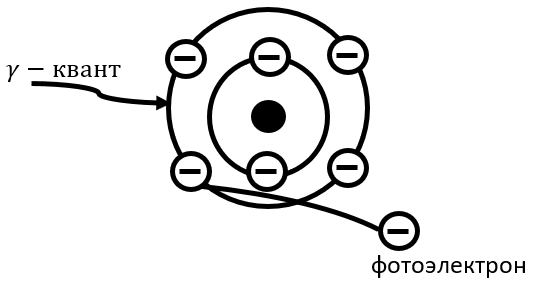
\includegraphics[width=.5\textwidth]{photoeffect.png}

\subsubsection{Эффект Комптона}
\emph{Эффект Комптона}~---~\textit{явление изменения длины волны рассеянного рентгеновского излучения, при его рассеянии на свободных электронах}. 

Эффект Комптона наблюдается в том случае, когда энергия фотонов много больше энергии связей электронов ($E_\text{ф}>>E_\text{св}$).

Эффект Комптона можно рассматривать как результат упругого соударения кванта с электроном. При этом квант отдает электрону не всю энергию, а лишь часть, причем сам он продолжает движение в качестве рассеянного кванта в новом направлении и с меньшей энергией. В отличие от фотоэлектрона, комптон-электрон (его еще называют электроном отдачи) приобретает не всю энергию первичного кванта. 
%TODO: вставить формулу фотоэффекта

В воде или биологических тканях поглощение излучения с $E=300$ кэВ в основном происходит за счет эффекта Комптона.

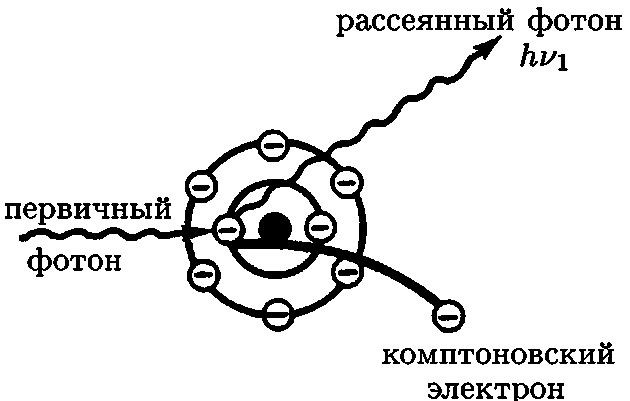
\includegraphics[width=.5\textwidth]{ComptonScattering.png}

\subsubsection{Образование электрон-позитронных пар}
Если энергия падающего кванта превышает $Е_\text{ф}>1,022$ МэВ, то становится возможным образование электронно-позитронных пар ($Е_0=0,511$ МэВ~---~энергия покоя электрона). 

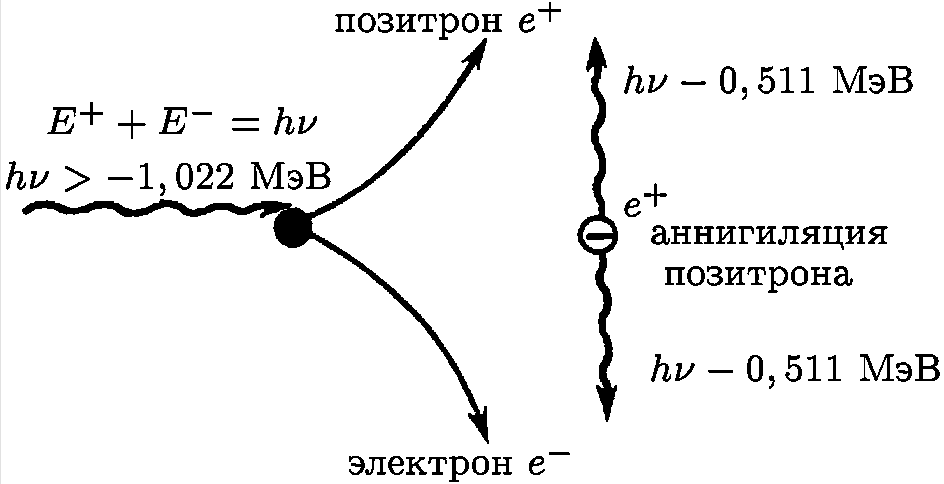
\includegraphics[width=.5\textwidth]{elPosCouple.png}

\textit{Электронно-позитронные пары образуются в результате взаимодействия кванта излучения с кулоновским полем ядра: квант с высокой энергией, приближаясь к полю ядра атома, исчезает, одновременно возникает пара элементарных частиц:} 
\[ h\nu \rightarrow e^{+} + e^{-}\]
Вся энергия падающего кванта используется на образование пары, причем энергия, равная 1,022 МэВ, всегда преобразуется в «массу покоя» элементарных частиц, а остаток~---~в их кинетическую энергию:
\[E_{\text{кин.}e^{-}}+E_{\text{кин.}e^{+}} = h\nu - 1,022\;\text{МэВ}.\]

Суммарную кинетическую энергию пары можно условно разделить поровну между электроном и позитроном, но в действительности она зависит от углов разлета этих частиц. Пролетающий через вещество позитрон испытывает взаимодействия с электронами среды, при этом происходит их аннигиляция. В результате образуется $\gamma$-квант, способный передать энергию веществу за счет комптоновского и фотоэффекта, а также ядро отдачи, которое обязательно получает свою порцию энергии за счет действия закона сохранения энергии. Вероятность рождения пары электрон-позитронувеличивается с ростом энергии кванта и пропорциональна $Z^2$. В биологических системах этот эффект выражен слабо, так как средний эффективный атомный номер $Z$ имеет малые значения.
\begin{figure}[htbp]
    \centering
    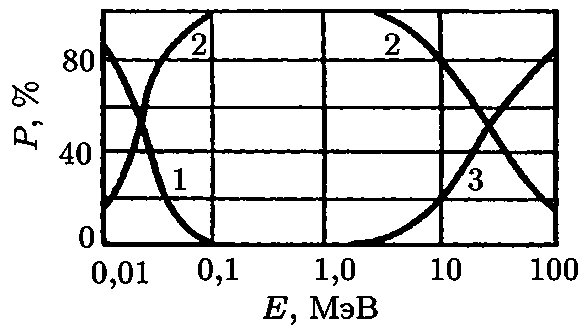
\includegraphics[width=.5\textwidth]{adsorptionShare.png}
    \caption{Доля механизма поглощения в зависимости от энергии фотона: 1~---~фотоэффект; 2~---~комптоновский эффект; 3~---~образование пар}
    \label{adsorptionShare}
\end{figure}

Как видно из рисунка \ref{adsorptionShare}, кванты с энергией 10~--~100 кэВ в биологических тканях
поглощаются преимущественно за счет фотоэффекта;

в диапазоне энергий 0,3~--~10 МэВ основной тип взаимодействия~---~эффект
Комптона, а при энергиях квантов более 10 МэВ начинает преобладать эффект
образования пары электрон-позитрон.

Аннигиляция пары приводит к образованию двух $\gamma$-квантов с энергией 0,511
МэВ.

Поглощение квантов электромагнитного излучения высокой энергии приводит к
возникновению в веществе небольшого числа атомов, утративших электроны. Эта
первичная ионизация~---~следствие фото- и комптоновского эффектов.
Высвободившиеся электроны обладают огромным запасом кинетической энергии (к
ним перенесена большая часть энергии падающего кванта) и могут многократно
взаимодействовать с атомами и молекулами, отдавая энергию на их ионизацию и
возбуждение. Так продолжается до тех пор, пока энергия свободного электрона не
снизится до того минимального уровня, при котором электрон уже сможет
присоединиться к нейтральному атому с образованием отрицательного иона.

Каждый первичный электрон от момента своего рождения до захвата
нейтральным атомом или молекулой многократно взаимодействует с атомами,
расположенными вдоль направления его движения, генерируя большое число
вторичных электронов. Распределение энергии вторичных электронов точно можетбыть рассчитано лишь для атома водорода. Для более сложных молекул возможны
лишь качественные рассуждения.

Перенос веществу энергии квантов излучения осуществляют главным образом
высокоэнергетические вторичные электроны. Первичная ионизация при действии
рентгеновского или -излучения пренебрежимо мала по сравнению с тем количеством
ионизированных и возбужденных атомов, которое возникает в результате
взаимодействия вторичных электронов с веществом. Поэтому фотоны рентгеновского
и $\gamma$-излучения следует относить к косвенно ионизирующим частицам,
высвобождающим в веществе непосредственно ионизирующие частицы~---~высокоэнергетические вторичные электроны.

\subsection{Механизм поглощения нейтронного излучения}
Нейтронное излучение – поток нейтронов, то есть частиц с массой равной 1,0087 а.е.м. и зарядом $q = 0$.

Нейтронное излучение в зависимости от энергии частиц делит их на быстрые,
медленные и промежуточные нейтроны.

Вследствие электронейтральности нейтроны не взаимодействуют с кулоновскими полями атомов и молекул и могут проходить в веществе значительные расстояния, не отклоняясь от первоначального направления. Нейтрон, не имея заряда, тем не менее вызывает ионизацию атомов и молекул. Происходит это за счет косвенных эффектов, связанных со следующими типами взаимодействия нейтронов с ядром атома.

\emph{I. Упругое рассеяние} результат соударения нейтрона с ядром атома. Кинетическая энергия нейтрона распределяется между ним и «ядром отдачи» согласно уравнению: 
\begin{equation}
    E = \frac{4m_\text{н}}{M+m_\text{н}}\cdot E_\text{н}\cos^2\theta, 
\end{equation}
где $m_\text{н}$ и $E_\text{н}$ – масса и энергия нейтрона, $М$ и $Е$ – масса и энергия ядра отдачи, $\theta$ – угол между направлением движения падающего нейтрона и ядра отдачи. Из уравнения следует, что ядру отдачи передается максимальная энергия, если это ядро имеет минимальную массу $М$. Значит, в результате упругого рассеяния наибольшее количество энергии нейтронного излучения поглощает водород (М = 1). 

\emph{II. Неупругое рассеивание} нейтронов состоит в том, что часть их энергии идет на сообщение ядру запаса кинетической энергии, а часть~---~на возбуждение ядра. А возбужденное ядро переходит в основное состояние с испусканием одного или нескольких γ-квантов. 

Неупругое рассеяние становится возможным при энергии нейтронов больше нескольких кэВ. В результате этого эффекта помимо непосредственно ионизирующих частиц (ядра элементов) в веществе возникают γ-кванты. 

\emph{III.} При низких значениях скоростей нейтронов возможен \emph{радиационный захват нейтрона ядром}.

Согласно уравнению Ферми: $\sigma_{(n,\gamma)} \sim \frac{1}{\sqrt{E_\text{н}}} \sim \frac{1}{\nu_\text{н}}$, где $E_\text{н}$ и $\nu_\text{н}$ – энергия и скорость нейтрона соответственно, $\sigma$ – эффективное сечение реакции, т. е. величина, количественно характеризующая вероятность взаимодействия нейтронов с ядром. 

В результате образуется короткоживущее высоковозбужденное ядро – компаунд-ядро и оно переходит в стабильное состояние с испусканием γ-квантов, протонов и α-частиц. 

При захвате нейтрона легкими ядрами, например ядром водорода, испускается γ-квант с энергией 2,2 МэВ: \ce{^{1}_{1}H + ^{1}_{0}e \rightarrow ^{2}_{1}D} + $\gamma$. Если же нейтрон захватывается промежуточным или тяжелым ядром, то могут испускаться протоны или α-частицы. Так, в случае захвата нейтрона ядром азота образуется изотоп углерода \ce{^{14}_{6}C} и испускается протон с энергией 0,66~МэВ: 
\[ \ce{^{14}_7N} + \ce{^1_0n} \rightarrow \ce{^{14}_6C} + \ce{^1_1p}\]
Соотношение каждого из перечисленных процессов поглощения нейтронного излучения зависит от энергии частиц. Таким образом, нейтрон можно отнести к разряду косвенно ионизирующих частиц и объединить их по принципу действия в одну группу с фотонами рентгеновского и γ-излучения. 

\emph{Косвенно ионизирующие частицы} – это незаряженные частицы, которые могут высвобождать непосредственно ионизирующие частицы или вызывать ядерные превращения.

\subsection{Ионизация в тканях косвенно ионизирующими частицами}
Нейтронное, рентгеновское и $\gamma$-излучение генерируют в веществе ионизации,
пространственное распределение которых существенно отличается от такового при
действии ускоренных заряженных частиц.

Электронейтральные частицы, обладая высокой проникающей способностью,
углубляются в ткани организма на значительные расстояния. Они формируют
большинство ионизации косвенным путем: фотоны рентгеновского и $\gamma$-излучения – за
счет комптоновских и фотоэлектронов, а нейтроны – за счет ядер отдачи. Эти
заряженные частицы в основном и осуществляют перенос энергии излучения
веществу, вызывая ионизации и возбуждения атомов.

Мягкие рентгеновские лучи (до 100 кэВ) поглощаются в поверхностных слоях
ткани за счет фотоэлектронов (фотоэффекта), длина пробега которых не превышает 2 мм. Именно поэтому биологический эффект возникает вблизи места поглощения падающего кванта.

Жесткие рентгеновские и γ-лучи (с энергией фотонов выше 300 кэВ)
взаимодействуют с тканями посредством эффекта Комптона. При этом максимум
выделения энергии лежит на глубине вплоть до нескольких сантиметров.

Так, $\gamma$-лучи \ce{^{60}_{27}Co} теряют 60\% всей энергии при прохождении первых 5~--~6 см ткани, а фотоны с энергией 35 МэВ, генерируемые в бетатронах, отдают максимум своей
энергии на глубине 6~--~8 см.
\begin{figure}[htbp]
    \centering
    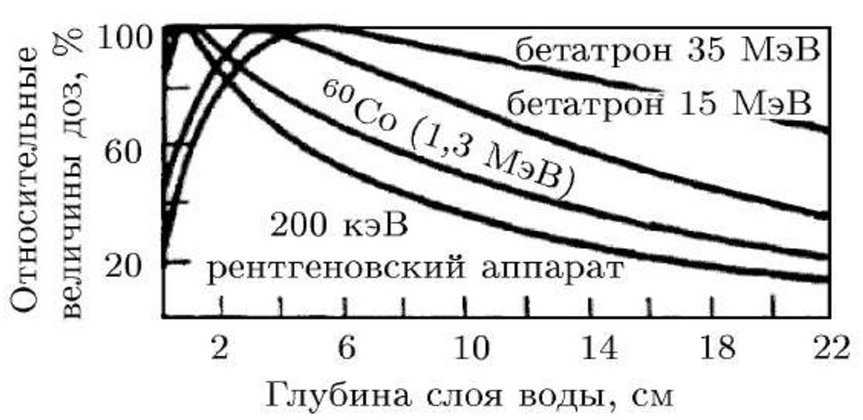
\includegraphics[width=.5\textwidth]{adsorbInWater.jpg}
    \caption{Поглощение энергии в воде для рентгеновского и $\gamma$-излучения  с разной энергией квантов}
    \label{adsorbInWater}
\end{figure}
Электроны, высвобождаемые квантами излучения на поверхности облучаемого объема, образуют максимальное число ионов на глубине ткани в несколько сантиметров, т.е. они осуществляют перенос энергии излучения вглубь ткани. 

На рисунке \ref{adsorbInWater} показан характер ионизации вещества жестким рентгеновским излучением при общей поглощенной дозе $10^4$ Гр. Облучение нейтронами высоких энергий (10~--~15 МэВ) приводит к пространственному распределению ионов в поглощающей ткани, которое сходно с картиной ионизации жестким γ-излучением. Отличие состоит в том, что энергия нейтрона переносится не к электронам, а к ядрам отдачи, т. е. к тяжелым ускоренным частицам, несущим положительный заряд. Наибольшее количество энергии переносится протонами отдачи, т. е. ускоренными ядрами водорода. 

Так, при облучении тканей такими нейтронами основная часть поглощенной дозы создается протонами и тяжелыми ядрами отдачи с высокой плотностью ионизации. В результате облучения тканей в редко расположенных микрообъемах возникают короткие треки с очень высокой плотностью ионизации. Это служит причиной значительно более высокого, чем для рентгеновского и γ-излучения, значения ОБЭ нейтронов высоких энергий.

\subsection{Поглощение ускоренных заряженных частиц}
Облучение тканей косвенно ионизирующими частицами в конечном счете
заканчивается появлением заряженных частиц: фотоны рентгеновского и $\gamma$-излучения
высвобождают в тканях высокоэнергетические электроны; нейтроны вызывают
появление в тканях протонов отдачи, $\alpha$-частиц и ядер других элементов. Все эти
заряженные частицы обладают значительной энергией и способны многократно
вызывать ионизацию и возбуждение атомов и молекул.

При возмущении атомов существует вероятность либо перехода их в
возбужденное состояние, либо их ионизации.

\emph{Следствия, к которым приведет наложение на атом дополнительного поля
заряженной частицы:}
\begin{enumerate}
    \item Действие поля ускоренной частицы вызывает временное возмущение каждого атома, вблизи которого частица проходит;
    \item Это возмущение существует тем больше, чем медленнее движется частица;
    \item Частицы, несущие не единичный заряд, вносят большее возмущение, чем однозарядные; 
    \item Величина массы движущихся частиц не влияет на количество перенесённой энергии, т. е. при равных скоростях электроны и протоны переносят веществу одинаковое количество энергии, хотя массы их различаются почти в две тысячи раз.
\end{enumerate}

\subsubsection{Уравение Бете-Блоха}
Вероятность взаимодействия отдельной частицы с веществом характеризуется
эффективным сечением взаимодействия. Обычно его пересчитывают на более
удобные для практического применения величины. Количественно дифференциальная
потеря энергии заряженной частицы, т. е. потери энергии на единицу длины трека (в
единицах МэВ/см), определяются из уравнения Бете-Блоха:
\begin{equation} \label{energyLoses}
    -\frac{d E}{d x}=\frac{4 \pi e^{4} z^{2} N Z}{m v^{2}}\left[\ln \frac{2 m v^{2}}{I_{0}}-\ln \left(1-\beta^{2}\right)-\beta^{2}\right]
\end{equation}
где $е = 1,602\cdot10^{-19}$ Кл~---~заряд электрона; $v$~---~скорость частицы в см/с; $z$~---~заряд
частицы в единицах элементарного заряда е; $N$~---~число атомов в 1 см$^3$ вещества; $Z$~---~среднее число электронов в атоме, т. е. «эффективный» атомный номер; $I_0$~---~средний
потенциал ионизации или возбуждения атома, определяемый экспериментально;
$\beta = \frac{v}{c}$ (отношение скорости заряженной частицы к скорости света); для того, чтобы
получить потери энергии в единицах МэВ/см, массу электрона принимают равной
= 0,511 МэВ/с$^2$. 
%TODO: добавить не релятивийский случай

Действительно, член $e^4z^2$ соответствует взаимодействию между полем
заряженной частицы и электроном (это становится яснее, если записать его в виде
$(e^2z)^2$, т. е. в виде квадрата произведения квадрата заряда летящей частицы на заряд
электрона в атоме).

Анализируя уравнение \ref{energyLoses}, можно количественно обосновать проведенные выше
качественные представления. Чем выше заряд, тем (больше) сильнее взаимодействие.
Зависимость от скорости определяется в основном первым множителем, в который
входит $\frac{1}{v^2}$, так как во втором множителе скорость частицы входит в медленно
изменяющуюся функцию, содержащую энергию $\frac{mv^2}{v^2}$ под знаком логарифма. В
формуле фигурирует только масса электрона как масса возбуждаемой в атоме
частицы.

\subsubsection{Пик Брегга}
Потеря энергии пропорциональна $NZ$, т. е. зависит от числа атомов в единице
объема и от числа электронов в атоме. По мере торможения частиц их энергетический
спектр размывается. Тем не менее наблюдается максимум, который известен как \emph{пик
Брегга}: \textit{резкое возрастание потерь энергии в конце пути заряженной частицы}.
\begin{figure}[htbp]
    \centering
    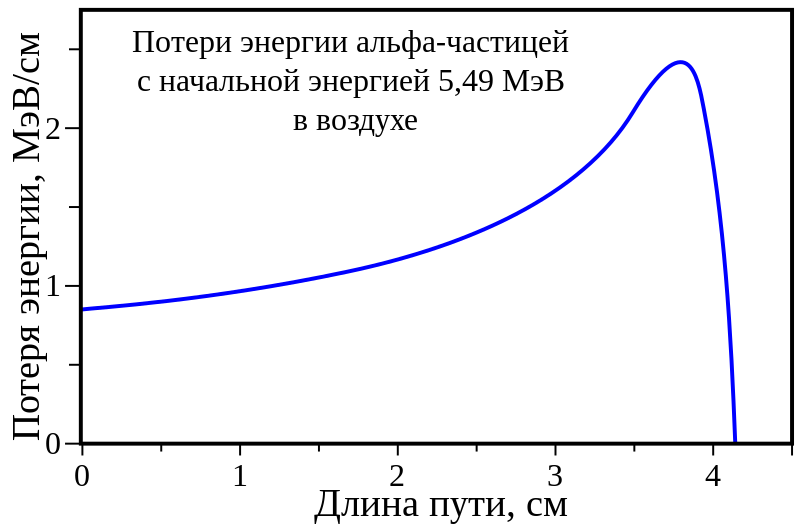
\includegraphics[width=.5\textwidth]{BraggPeak}
    \caption{Плотность ионизации в зависимости от пройденного пути}
    \label{Breg'sPeak}
\end{figure}
На рисунке \ref{Breg'sPeak} показано резкое возрастание удельных потерь энергии $\frac{dE}{dx}$ в конце пути заряженных частиц (пик Брэгга).

Подбирая соответствующий тип излучения и варьируя энергию ионизирующих частиц, можно добиться оптимального распределения поглощенной дозы, в частности, благоприятного соотношения между степенью поражения нормальных тканей и опухолей, залегающих на значительной глубине (Рис. \ref{spaceDistribution}).

% При лечении опухолей используются специальные фильтры, чтобы добиться нужной ширины и глубины пика Брегга 

\begin{figure}[htbp]
    \centering
    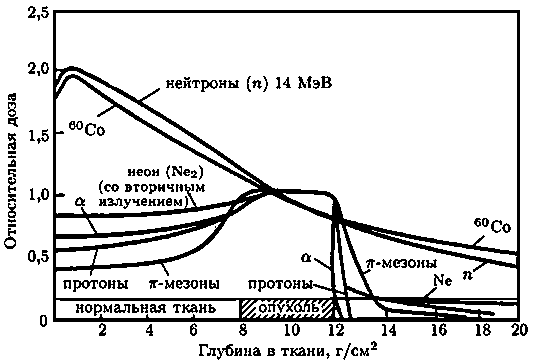
\includegraphics[width=.7\textwidth]{SpaceDistibution.png} %TODO: Поменять рисунок
    \caption{Пространственное распределение поглощенной дозы для разных видов излучения}
    \label{spaceDistribution}
\end{figure}

Существование пика Брэгга позволяет с максимальной эффективностью проводить лучевую терапию злокачественных опухолей. 

В зависимости от локализации опухолей выбирают вид излучения и его энергетическую характеристику такими, чтобы пик Брэгга приходился на топографически обозначенный очаг злокачественных клеток.

\section{Зависимость биологического эффекта от поглощенной дозы излучения.
Кривые доза-эффект}

Первые количественные эксперименты были проведены в конце 20-х гг. XX
века. Этому способствовало:

\emph{Во-первых}, широкое распространение получают ионизационный метод
дозиметрии излучения и использование в качестве единицы экспозиционной дозы
рентгена. Благодаря этому облучение экспериментальных объектов становится строго
дозированным, и условия опыта могут быть многократно воспроизведены.

\emph{Во-вторых}, для количественных экспериментов радиобиологи стали
использовать клоны генетически однородных клеток, вирусные частицы, препараты
макромолекул, т. е. такие системы, в которых легко определить реакцию единичного
объекта на действие излучения в данной дозе.

Уже в первых радиобиологических исследованиях отмечалась важнейшая
закономерность~---~вероятностная природа проявления реакции клеток на облучение.
При оценке зависимости доли погибших клеток от величины дозы облучения
выяснялось, что различные одноклеточные объекты гибнут при самых малых дозах
облучения, с ростом дозы увеличивается число погибших клеток, однако даже при
облучении в очень высоких дозах некоторое число клеток сохраняет
жизнеспособность.

Существенно, что с ростом дозы облучения наблюдалось увеличение не столько
степени проявления эффекта (глубины поражения отдельной клетки), сколько доли
летально пораженных клеток в облученной популяции.

\emph{Кривые доза-эффект}~---~\textit{зависимость доли выживших клеток от величины дозы
облучения.}

Для построения кривых определенное количество объектов данного вида
облучали в широком диапазоне волн и после облучения определяли дозу той доли
объектов.

Из этих кривых было видно, что при самых малых дозах облучения часть клеток
гибнет.

В настоящее время установлено, что при облучении в малых дозах наблюдается
более сложная немонотонная зависимость дозы-эффект.

При больших дозах некоторая часть клеток сохраняет свою жизнеспособность.
Обычно такие кривые носят экспотенциальный характер. %TODO: экспотенциальный?

Для объяснения вида кривых использовались представления о том, что реакция
клеток на облучение носит вероятностный характер, а также об особенности
воздействия ионизирующих излучений на организм, а именно \textit{о дискретной природе
передачи энергии ионизирующего излучения атомом-поглотителем}.

Объяснение наблюдаемого вида кривых зависимости эффекта от дозы
облучения все же следует искать в особенностях воздействия ионизирующих
излучений, в способе сообщения ими энергии биологическому объекту, т. е. в иной,
биофизической трактовке экспериментальных кривых «доза-эффект».

\subsection{Гипотеза точечного нагрева}
В начале 20-х гг. Дэссауэр выдвинул гипотезу точечного нагрева, которая
основывалась на следующих положениях:
\begin{enumerate}
    \item ионизирующие излучения обладают очень малой объемной плотностью по
    сравнению с видимым или ультрафиолетовым светом энергетически эквивалентной
    дозы;
    \item фотоны рентгеновского или $\gamma$-излучения, ускоренные электроны или
    тяжелые заряженные частицы обладают огромной энергией, величина которой
    значительно превосходит энергию любой химической связи;
    \item облучаемый биологический объект, например клетка, состоит, с одной
    стороны, из относительно менее значимых и, с другой – весьма существенных для
    жизни микрообъемов и структур;
    \item в облучаемом объекте при поглощении относительно небольшой общей энергии в отдельных случайных и редко расположенных микрообъемах остаются
    настолько большие порции энергии, что их можно сравнить с микролокальным
    нагреванием и они могут производить почти любые узколокальные изменения в
    веществе;
    \item так как распределение «точечного тепла» является чисто статистическим,
    то конечный эффект в клетке будет зависеть от случайных попаданий дискретных
    порций энергии в жизненно существенные микрообъемы внутри клетки. С
    повышением дозы увеличивается вероятность таких попаданий, и наоборот, при
    понижении дозы вероятность снижается. Из этого следует, что любая самая малая доза
    может соответственно с малой вероятностью и, следовательно, малой частотой
    вызывать экстремальный биологический эффект (например, гибель клетки), но даже
    при очень высокой дозе могут с малой вероятностью и малой частотой сохраниться
    отдельные неповрежденные клетки.
\end{enumerate}

В 1922г. Блау и Альтенбургер предложили \textit{общую формулу для расчета кривых
дозы-эффект, основанную на принципе «попадания»}:
\begin{equation}
    \frac{N}{N_{0}}=1-e^{-\nu D} \sum_{k=0}^{k=n-1} \frac{(\nu D)^{k}}{k !}
\end{equation}
где $N0$ – исходное число клеток до облучения, $N$ – число клеток, прореагировавших
данным образом, $D$ – доза облучения, $n$ – требуемое число попаданий в мишень и $\nu$ – коэффициент, пропорциональный объему $V$ «мишени», попадание в которую
приводит к оцениваемому эффекту (точный смысл коэффициента $\nu$ будет определен
при рассмотрении статистики одноударных процессов).

Блау и Альтенбургер рассчитали теоретически кривые доза-эффект для разного числа
попадания в мишень, эти кривые соответствовали реальным кривым, наблюдаемым
при облучении изолированных клеток.

\subsection{Принцип попадания и его основные физические принципы. Концепция мишени}
\emph{Принцип попадания и теория мишени} были предложены рядом ученых:
Кроутер, Ли, Тимофеев-Рессовский.

В 1924 г. Кроутер первым сформировал принцип попадания. Он предположил,
что регистрируемый эффект связан с некоторым критическим числом ионизации
(попаданий) в пределах мишени, занимающей определенный чувствительный объем
внутри клетки. Параметры мишени оказались сопоставимыми с размерами центриолей
и ядрышек.

С тех пор в радиобиологии начался активный поиск мишени на основании
статистических принципов попадания. Он привел к выводу о ведущей роли ядра и
внутриядерных наследственных структур в летальном поражении клетки.

\subsubsection{Одиночные и множественные попадания в мишень}
Количественный анализ, основанный на принципе попадания, состоит в том, что кривые «доза-эффект» интерпретируются на основе следующих физических положений:
\begin{itemize}
    \item Ионизирующее излучение переносит энергию в дискретном виде;
    \item Акты взаимодействия (попадания) не зависят друг от друга и подчиняются
    пуассоновскому распределению;
    \item Исследуемый эффект наступает, если число попаданий в некоторую
    чувствительную область гетерогенной биологической структуры, так называемую
    мишень, составляет по крайней мере $n \geqslant 1$.
\end{itemize}
Рассмотрим простейший случай \emph{«одноударного процесса»}, когда попаданием
считают одиночную передачу некоторого минимального количества энергии.
Тестируемый эффект наступает лишь тогда, когда определенное минимальное
количество энергии поглощено чувствительной областью – мишенью.

Пусть облучаемая система состоит из $N_0$ объектов, каждый из которых обладает
мишенью сечением $S$ и объемом $V$. Пусть для инактивации объекта достаточно, чтобы
трек плотно ионизирующей частицы прошел через сечение мишени $S$; такое событие
будем именовать попаданием.

Если траектории частиц распределяются по поперечному сечению объекта
случайным образом и не зависят друг от друга, то вероятность \emph{одного, двух, ..., n}
попаданий в мишень, находящуюся в пределах объекта, описывается уравнением:
\begin{equation}
    P(n) = \frac{\alpha^ne^{-\alpha}}{n!},
\end{equation}
где $alpha$ – среднее число попаданий в мишень. Если \textit{Ф} – флюенс, то есть
среднее число частиц, пролетающих через единичную площадку, a $S$ – сечение
мишени, то $\alpha$ = 5~Ф. Как было определено формулой $D = 1,602\cdot 10^{-1}\cdot L\text{Ф}$ (см. ур-ние \ref{adsorbDoze}), где \textit{Ф} (отношение \textit{dN/dS}) флюенс пропорционален поглощенной дозе излучения.

С увеличением потока частиц (т.е. с ростом дозы излучения) в объекте
возрастает число мишеней, в которые произошло попадание.

Если $N_0$ – общее число объектов в облучаемой системе, $N$ – общее число
объектов, сохранивших после облучения исходные свойства, то величина $\frac{N}{N_0}$
соответствует вероятности непопадания ($n=0$). Из предыдущего уравнения для случая
$n=0$ (учитывая, что $0! =1$) получим 
\begin{equation} \label{hitProbability}
    \frac{N}{N_0} = \frac{(S\text{Ф})^0 e^{-S\text{Ф}}}{0!} = e^{-S\text{Ф}}.
\end{equation}

При некоторой дозе облучения выполняется условие $S\text{Ф} = 1$. Это соответствует
случаю, когда в среднем число попаданий равно числу мишеней. В действительности
же часть попаданий испытали уже однажды пораженные мишени, а некоторые не
претерпели ни одного попадания.

Согласно формальной статистике Пуассона при $S\text{Ф} = 1$ реально поражается
только 63\% мишеней, а 37\% оказываются непораженными (Здесь не учитываются
процессы восстановления в облученных клетках). Действительно, подставив в
уравнение \ref{hitprobability} значение $S\text{Ф} = 1$, получим
\[ \frac{N}{N_0} = e^{-S\text{Ф}} = e^{-1} = 0,37.\]
Из соотношения \ref{hitprobability} с учётом формулы \ref{adsorbDoze} определяется и доза облучения, при которой выживает 37\% объектов ($N/N_0 =0,37$).

Отношение $N/N_0$ легко определить в эксперименте: это доля «выживших»
объектов по отношению к их общему числу до облучения. Узнав, при какой дозе
облучения выживает 37\% объектов, т.е. $N/N_0 = 0,37$ (эту дозу излучения обозначают
символом $D_{37}$), мы можем определить сечение мишени, принимая, что дозе $D_{37}$
соответствует флюенс Ф$_{37}$ который определяется формулой \ref{adsorbDoze}: $S\text{Ф}_{37} =1, S =1/\text{Ф}_{37}$.

\begin{figure}[htbp]
    \centering
    \includegraphics[width=\textwidth]{adsorbScheme.png}
    \caption{Cхема, иллюстрирующая зависимость числа пораженных
    мишеней от дозы облучения: 1 – объект с мишенью сечением $S$; 2 – треки частиц}
    \label{adsorbScheme}
\end{figure}
Из рисунка \ref{adsorbScheme}-a видно, что даже при облучении в малой дозе
некоторое число частиц проходит через мишени и вызывает их инактивацию. С
ростом дозы число пораженных объектов возрастает резко, почти линейно, а затем все
более вероятно повторное прохождение частиц через уже пораженные мишени. При
дозе $D_{37}$ (рис. \ref{adsorbScheme}-б) общее число частиц соответствует числу мишеней ($SD =1$), но 37\% объектов остаются непораженными, тогда как некоторые из 63\% мишеней испытали по два и более попаданий.

Даже при очень большой дозе облучения все же какое-то число объектов оказалось не пораженным излучением (рис. \ref{adsorbScheme}-в). Графически зависимость доли выживших клеток от величины дозы выражается экспонентой (рис. \ref{adsorbScheme}-г): $\frac{N}{N_0} = e^{-S\text{Ф}} = e^{-\frac{D}{D_{37}}}$.

Экспоненциальная зависимость доза-эффекта это важный, но не единственный
критерий одноударности процессов инактивации. Если в действительности одного
попадания в мишень достаточно для инактивации объекта, то должны выполняться
следующие требования:
\begin{enumerate}
    \item эффект, вызываемый облучением в данной дозе, не зависит интенсивности
    излучения (мощности дозы) и от того, какими частями доза сообщалась объекту;
    \item при одинаковом эффекте вызывающая его доза в различных излучениях
    возрастает при переходе от редко- к плотноионизирующим частицам.
\end{enumerate}
Если выполняется первое требование, значит тестируемый эффект не возникает
в следствии кумулятивного действия нескольких последовательных ионизации (иначе
эффект зависел бы от распределения ионизации во времени).

Каждая ионизация, возникающая в пределах облучаемых объектов, имеет
определенную вероятность оказаться причиной эффекта, но эта вероятность при
одноударном процессе не должна зависеть ни от времени, прошедшего с момента
предыдущей ионизации, ни от времени, отделяющего ее от последующей ионизации.

Следовательно, эффект данной дозы должен определяться только ее величиной
(т.е. числом возникших актов ионизации); интенсивность излучения и распределение
дозы во времени не должны играть никакой роли.

Выполнение второго требования означает, что плотноионизирующие излучения
менее эффективны, чем редкоионизирующие. Действительно, если одиночной
ионизации достаточно для возникновения тестируемого эффекта, то частицы,
производящие большое число ионов на единицу пути, вызовут в пределах мишени
множество «ненужных» ионизации. Редкоионизирующие излучения генерируют
сгустки ионов, значительно удаленные друг от друга, и вероятность возникновения
нескольких ионизации в пределах мишени малого размера незначительна. То при
одноударном процессе большинство попаданий вызываемых
плотноионизируирующим излучением бесполезны. Величина поглощенной дозы
определяет общее число ионизации, произведенных данным видом излучения в
единице объема. При одноударном процессе большинство ионизации, вызванных
плотноионизирующим излучением, «бесполезно». Поэтому при равной дозе, т. е. при
равном общем числе ионизации, редкоионизирующие излучения окажутся более
эффективными.

Напротив, если тестируемый эффект наступает вследствие большого числа ионизации в пределах мишени (многоударный механизм инактивации), то частицы с высокой плотностью ионизации окажутся значительно эффективнее, чем редкоионизирующие.

\begin{figure}[htbp]
    \centering
    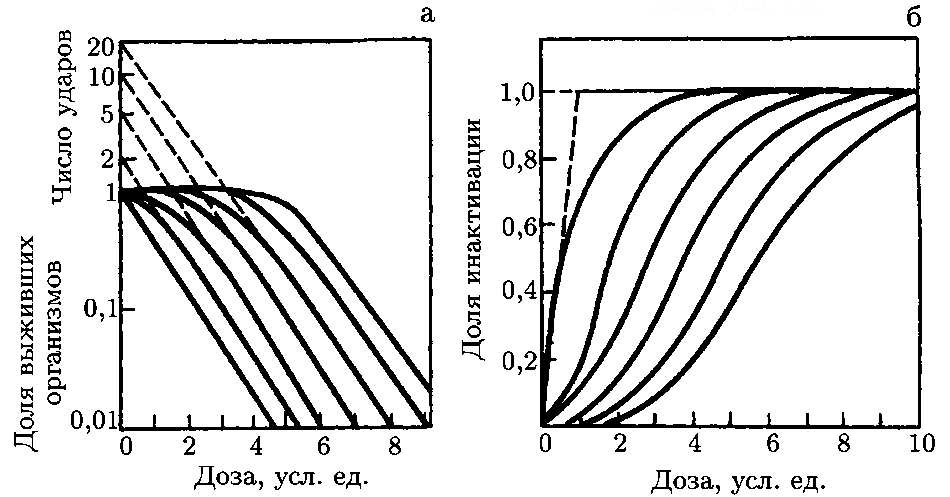
\includegraphics[width=\textwidth]{DozeCurveFamily.png}
    \caption{Семейство кривых доза-эффект}
    \label{DozeCurveFamily}
\end{figure}
Кривые «доза-эффект» при многоударном механизме инактивации отличаются
от экспоненциальных дозовых кривых, наблюдаемых в случае одноударного процесса.
В полулогарифмическом масштабе семейство дозовых кривых для случая $n =2, 3, ..., k$
представлено на рисунке \ref{DozeCurveFamily}-а в полулогарифмическом масштабе (обозначена
«Ударность» процесса инактивации); на рисунке \ref{DozeCurveFamily}-б в обычном масштабе.

Чем больше «ударность» мишени, тем заметнее «плечо»~---~начальный, более
горизонтальный участок кривой. Вслед за плечом следует переход к прямолинейному
участку, наклон которого совпадает с наклоном соответствующей одноударной
кривой.

Вид дозовой кривой при многоударном механизме инактивации определяется
тем, что при малых дозах лишь небольшое число объектов может испытать требуемое
число попаданий \emph{k}, а все остальные – не более \emph{k-1} попаданий. По достижении \emph{k-1}
попаданий во все или большинство объектов возникает ситуация, при которой
последнее, \emph{k-e}, попадание приводит к тестируемому эффекту. Начиная с этой дозы
кривая принимает вид, характерный для одноударного процесса.

На основании принципа попадания и концепции мишени можно анализировать
кривые «доза-эффект», полученные в эксперименте. В зависимости от вида объекта и
характера излучения получают различные дозовые кривые – от простых
экспоненциальных до сигмоидальных с различной шириной плеча. Подобное
применение принципа попадания позволило впервые определить размеры некоторых
макромолекул, вирусов, генов, получить сведения о внутренней структуре
бактериальных спор и т. д.

\section{Прямое и косвенное действие ионизирующего излучения. Этапы
биофизического анализа радиационной инактивации молекул}

В результате облучения макромолекул их биологические функции могут
полностью или частично утрачиваться. В этом случае говорят об инактивации
макромолекул ионизирующей радиацией. Инактивация макромолекулы может
произойти в результате прямого либо опосредованного действия ионизирующего
излучения.

\emph{Прямое действие} состоит в том, что инактивированными оказываются те
молекулы, которые непосредственно поглотили энергию излучения.

Если же молекула была поражена активными реакционноспособными
продуктами, возникшими за счет поглощения энергии излучения ее микроокружением
(например, полярными или неполярными растворителями), то говорят о непрямом
(опосредованном, косвенном) действии радиации.

Биофизический анализ механизмов лучевой радиационной инактивации
макромолекул состоит в описании в терминах физики и химии всей
последовательности процессов, которые начинаются с поглощения молекулой
дискретной порции энергии излучения и заканчиваются очевидными, доступными
экспериментальному анализу изменениями ее биологических свойств. Такой анализ
включает следующие \emph{три логически связанных этапа}.

\emph{Первый этап} – это феноменологический анализ картины лучевого поражения
молекул. Он осуществляется путем построения кривых «доза-эффект» и изучения на
их основе радиочувствительности отдельных биологических функций макромолекул.

В толковании понятия «биологические функции макромолекул» существует
известная неопределенность, связанная с тем, что в настоящее время мы не в
состоянии очертить весь круг функциональных признаков, определяющих уникальную
роль данного типа молекул в жизнедеятельности клеток и организмов. Еще труднее
охарактеризовать эти признаки количественно.

Однако для некоторых биомолекул уже сейчас можно указать на ряд свойств,
определяющих их значение в процессах обмена веществ, в хранении и передаче
наследственных свойств, в возникновении естественной изменчивости. Анализируя
влияние облучения на ферменты, мы прежде всего должны оценить изменения их
каталитической активности, субстратной специфичности, чувствительности к
соответствующим активаторам и ингибиторам, возможность воздействия на их
стерическое регулирование. Если по любому из этих функциональных признаков
отмечается негативный эффект облучения, то мы будем называть такое событие
лучевой инактивацией фермента. Соответствующими биохимическими методами
можно оценить степень инактивации количественно.

В экспериментах по облучению нуклеиновых кислот критерием инактивации
ДНК может служить изменение ее инфекционности, трансформирующей активности
(для бактериальных и вирусных ДНК), способности служить матрицей для синтеза
соответствующих комплементарных полинуклеотидных последовательностей.
Влияние излучения на молекулы тРНК оценивают по их способности связывать
специфические аминокислоты. В подобных опытах удается количественно оценить
инактивирующее действие излучения на этот тип нуклеиновых кислот.

На \emph{втором этапе} биофизического анализа механизмов радиационной
инактивации макромолекул последовательно оценивают стадии прямого эффекта
ионизирующей радиации (условно они делятся на первичную физическую, физикохимическую и химическую-деструктивную).

На \emph{третьем этапе} биофизического анализа устанавливаются причинноследственные связи между типами структурного повреждения и характером инактивации макромолекулы. Для решения этих вопросов перспективно использование модифицирующих агентов, видоизменяющих типы структурного
повреждения и (или) характер инактивации. Сочетание различных модифицирующихагентов позволяет дифференциально оценить роль тех или иных типов повреждений в
инактивации макромолекулы.

Детальное описание всех этапов радиационной инактивации макромолекул
составляет одну из важнейших задач современной радиационной биофизики. Эта
проблема еще далека от полного разрешения.

Однако уже сегодня можно говорить о важнейших деталях и указать основные
направления, по которым развиваются исследования.

% \section{Феноменологический анализ картины лучевого поражения макромолекул.
% Прямое действие излучения на ферменты: эксперимент. зависимости,
% сравнение радиочувствительности функций ферментов. Доза Д$_{37}$} %TODO: надо бы назвать этот раздел локаничнее
\section{Феноменологический анализ картины лучевого поражения макромолекул}
Прямое действие ионизирующей радиации на макромолекулы обычно
исследуют на обезвоженных или кристаллических препаратах ферментов и
нуклеиновых кислот. 
В этом случае большинство молекул инактивируется в
результате прямого поглощения энергии излучения (Следует все же оговориться, что
даже при облучении высокоочищенных препаратов в глубоком вакууме наличие
одного только прямого действия маловероятно: активные продукты, возникающие при
поражении одних молекул, могут индуцировать структурные изменения в молекулах
ближайшего окружения.)

\subsection{Прямое действие излучения на ферменты}

Схема эксперимента по определению числа инактивированных молекул
фермента при действии излучения в данной дозе состоит в том, что ампулу с
гомогенным препаратом (сухим или кристаллическим) подвергают облучению, а затем
сопоставляют активность опытного и контрольного образцов. 
Путем соответствующего пересчета можно перейти от доли инактивированных молекул (или
процента инактивации) к истинному числу молекул фермента, инактивированных
излучением в данной дозе. Используя соответствующие биохимические методы,
можно оценить изменение различных функциональных свойств облученного фермента – каталитической активности, субстратной специфичности, стерического регулирования и т. д.
\begin{figure}[htbp]
    \centering
    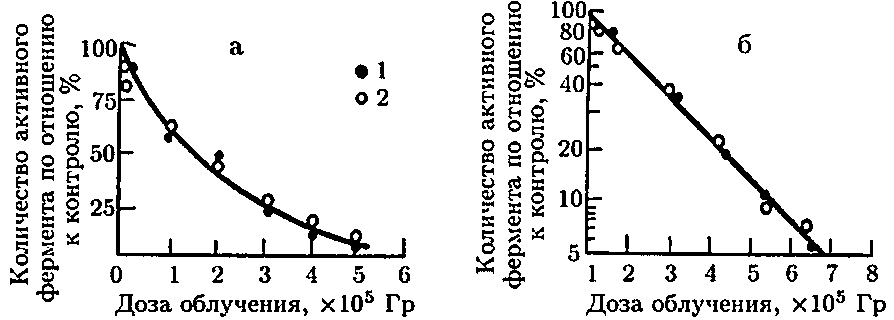
\includegraphics[width=.8\textwidth]{inactivationOfFerment.png}
    \caption{Инактивация РНКазы $\gamma$-излучением. Ферментная активность определялась для     двух различных субстратов: 1 – РНК; 2 – цитидин-2', 3'-циклофосфата; а) зависимость «доза-эффект» выражена в линейных координатах; 6) эти же данные представлены в полулогарифмическом виде, экспериментальные точки укладываются на прямую}
    \label{inactivationOfFerment}
\end{figure}
На рис. \ref{inactivationOfFerment} представлены результаты одного из экспериментов Юнга и
Дертингера с кристаллической рибонуклеазой. В широком диапазоне доз излучения
оценивается каталитическая активность и субстратная специфичность облученного
фермента.

Так как деградация РНК под действием рибонуклеазы осуществляется в два
этапа (вначале расщепляется фосфодиэфирная связь в РНК и образуется циклический
диэфир, а на второй стадии фосфатная связь гидролизуется до нуклеотид-3-фосфата),
то, используя РНК в качестве субстрата, можно исследовать суммарную реакцию, а с
помощью цитидин-2', 3-циклофосфата – только вторую ее стадию.

Одинаковую радиационную инактивацию РНКазы наблюдали при использовании обоих субстратов (рис. \ref{inactivationOfFerment}), т.е. при облучении в равной мере поражаются обе функциональные единицы фермента.

% Зависимость эффекта от дозы облучения экспоненциальна.
При самых малых дозах обнаруживаются молекулы фермента, утратившие
способность расщеплять субстраты обоих типов. С ростом поглощенной дозы число
таких молекул возрастает вначале резко, почти линейно, а затем мы видим, как
значительному приращению дозы соответствует лишь небольшое увеличение доли
инактивированных молекул (рис. \ref{inactivationOfFerment}-а).

Экспоненциальный характер зависимости «доза-эффект»
подверждает построение кривой в полулогарифмических
координатах\footnote{По оси ординат откладывается не доля
молекул, сохранивших исходную активность, а натуральный логарифм этой
величины} (рис. \ref{inactivationOfFerment}-а). Все экспериментальные точки укладываются на прямую, проходящую под углом к оси ординат, следовательно, $ln\frac{N}{N_0} = -kD$ или $N/N_0 = e^{-kD}$.

Экспоненциальная зависимость «доза-эффект» обнаружена в экспериментах по
лучевой инактивации различных ферментов и может рассматриваться как общая
закономерность прямого действия радиации на ферменты~(рис. \ref{radioSensibility}).
\begin{figure}[htbp]
    \centering
    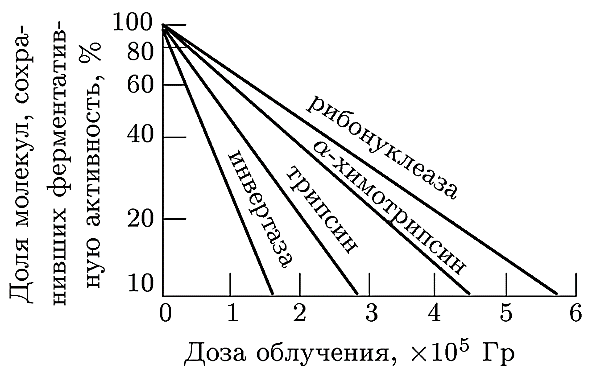
\includegraphics[width=.8\textwidth]{radioSensibility.png}
    \caption{Радиочувствительность ряда ферментов, подвергнутых воздействию $\gamma$-излучения в вакууме}
    \label{radioSensibility}
\end{figure}

Сравнивая кривые «доза-эффект», можно сопоставить радиочувствительность
различных ферментов. Из рисунка \ref{radioSensibility} видно, что для получения сравнимой инактивации изученных ферментов требуется существенно различающиеся дозы. Обычно в
качестве критерия радиочувствительности выбирают такую дозу излучения, которая
необходима, для инактивации 63\% молекул в облученном препарате фермента. Так
как при этом 37\% молекул сохраняют нативные свойства, эта доза получила название«доза 37\%-ой сохранности», или доза $D_{37}$. По рисунку можно установить, что для
инвертазы $D_{37}$ в данных условиях составляет около 80 кГр, а для рибонуклеазы – 280
кГр, т.е. при одинаковой дозе молекулы первого фермента поражаются со значительно
большей вероятностью. Это может быть связано с различными размерами
макромолекулы, особенностями ее аминокислотного состава, характером миграции
энергии в полимере или другими причинами, которые должны быть установлены в
ходе биофизического анализа.

Известно, что функциональные свойства фермента определяются его
различными структурными участками. Так как поглощение энергии излучения может
приводить к различным типам структурного повреждения, следует ожидать, что не все
функции фермента подавляются радиацией в равной степени. В таблице \ref{sensibilityOfFunstions} сведены результаты исследований различных авторов, которые подтверждают такую
возможность.
\begin{table}[htbp]
    \centering\begin{tabular}{|p{3,5cm}|C{12cm}|}
        \hline
        \emph{Фермент} & \emph{Радиочувствительность функций, связанных с ферментативной активностью (по величине дозы $D_{37}$)} \\ \hline
        химотрипсин & эстераза > протеаза > связывание диизопропилфосфата > уменьшение максимальной скорости > увеличение константы Михаэлиса-Ментен\tablefootnote{Более выскокая радиочувствительность (т.е. меньшие дозы $D_{37}$) обозначена символом \emph{>}. Например, эстераза > протеаза означает, что эстеразная активность фермента более радиочувствительная, чем протеазная} \\ \hline
        трипсин & протеаза > эстераза \\ \hline
        глутамат-дегидроденаза & уменьшение маскимальной скорости и увеличение константы Михаэлиса-Ментен > поражение активного центра и способности связывать кофермент\\ \hline
        рибонуклеаза & уменьшение маскимальной скорости; константы Михаэлиса-Ментен без изменения \\ \hline
        аспартаткарбамоилтрансфераза & поражение активного центра > инактивация участка ингибирования по принципу обратной связи (аллостерические свойства)\\ \hline
    \end{tabular}
    \caption{Радиочувствительность функций, определяющую биологическую активность ферментов}
    \label{sensibilityOfFunstions}
\end{table}

В опытах с рибонуклеазой обнаружено, что облучение приводит к снижению
максимальной скорости реакции, а величина константы Михаэлиса-Ментен остаетсябез изменения. Это означает, что число каталитически активных молекул в
облученном препарате понижается, однако пораженные молекулы сохраняют сродство
к субстрату. Вероятно, возникающие поражения структуры затрагивают активный
центр, но не препятствуют взаимодействию фермента со специфическим субстратом.
В случае с трипсином протеазная активность поражается в большей мере, чем
эстеразная, т.е. в результате облучения возникают повреждения главным образом в тех
структурных звеньях, которые определяют протеазную активность фермента.

Если ионизирующие излучения в состоянии вызывать специфические
структурные повреждения в молекуле фермента и приводить к определенному
изменению его функциональных характеристик, то с помощью радиационного
воздействия можно исследовать причинную связь между структурой и функцией
фермента.

Рассмотрение феноменологии лучевого поражения ферментов позволяет
заключить, что в результате прямого действия излучения возникают различные
нарушения функциональных свойств фермента; наблюдается экспоненциальная
зависимость биологического эффекта от величины поглощенной дозы, т.е. с
увеличением поглощенной дозы излучения доля макромолекул, сохранивших
нативные свойства, убывает по закону $e^{-kD}$, где \emph{k} – константа, \emph{D} – поглощенная доза. Облученный фермент может утрачивать одни функциональные свойства при
сохранении других, т.е. наблюдается неодинаковая радиочувствительность различных
биологических свойств фермента; по одному и тому же критерию, например
каталитической активности, различные ферменты обладают неодинаковой
радиочувствительностью.

\subsection{Прямое действие излучения на нуклеиновые кислоты.}
Существуют определенные трудности количественного измерения инактивации
нуклеиновых кислот. Существует ряд модельных систем позволяющих количественно
оценить важнейшие из функциональных характеристик этих макромолекул:
\begin{itemize}
    \item \textit{инфекционность нуклеиновых кислот;}
    \item \textit{трансформирующая активность;}
    \item \textit{затравочная активность мДНК;}
    \item \textit{способность ДНК к образованию гибридов мРНК;}
    \item \textit{способность т-РНК связывать соответствие аминокислоты;}
    \item \textit{функциональная активность рибосом.}
\end{itemize}
Их и основные феноменологические данные, полученные при изучении
характера инактивации облученных нуклеиновых кислот, мы рассмотрим подробно.

\subsubsection{Инфекционность нуклеиновых кислот}
Термином «инфекционность» обозначают способность вирусной ДНК или РНК
индуцировать образование бактериальной клеткой новых полноценных фагов.
Методически эксперимент выглядит так. Бактерии обрабатывают лизоцимом, в
результате чего они теряют часть клеточной стенки и образуют сферопласты, которые
можно инфицировать нуклеиновой кислотой, выделенной из бактериофага.
\begin{figure}[htbp]
    \centering
    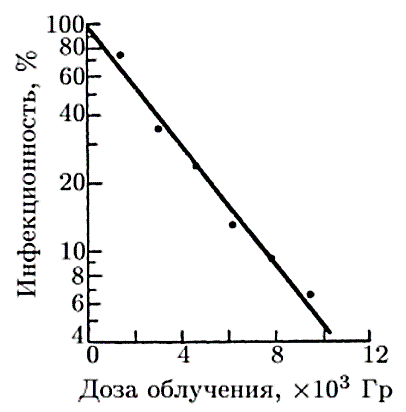
\includegraphics[width=.5\textwidth]{infectivityOfDNA.png}
    \caption{Инфекционность ДНК фага $\omega X174$, препарат которого подвергнут воздействию $\gamma$-излучению \ce{_{27}^{60}Co} в вакууме}
    \label{infectivityOfDNA}
\end{figure}
Если в инфицированной бактерии возникают новые полноценные фаги, то бактериальная стенка ее разрывается, и из бактерии высвобождается 100~--~200 бактериофагов. Количество вирусных частиц, высвободившихся из лизированных сферопластов, в определенных пределах пропорционально количеству молекул ДНК или РНК, сохранивших инфекционные свойства. Так как фаги лизируют новые сферопласты вблизи места своего высвобождения, то на сплошном газоне бактериальных клеток, выращенных на агаре, образуется пятно лизиса – «бляшка». Количество бляшек можно подсчитать визуально, и их число служит количественным критерием инфекционности вирусной нуклеиновой кислоты. 

Этим методом определяют инактивацию вирусной ДНК в результате облучения. Результаты одного из таких экспериментов приведены на рисунке \ref{infectivityOfDNA}. Доля молекул ДНК, сохранивших инфекционность, отложена по оси ординат в логарифмическоммасштабе, все экспериментальные точки укладываются на прямую, т.е. $ln \frac{N}{N_0} = -kD$, кривая «доза эффект» экспоненциальна.

\subsubsection{Трансформирующая активность}
Трансформирующая активность бактериальной ДНК часто оценивается по
появлению специфических генетических маркеров у бактерий-реципиентов,
«поглотивших» трансформирующую ДНК донора. Например, извлекают ДНК из
бактерии, устойчивой к стрептомицину, и клетки стрептомицин-чувствительных
мутантов инкубируют в ее присутствии. Если в результате этого путем рекомбинации
происходит встраивание специфической последовательности нуклеотидов ДНС
донора в геном реципиента, т.е. мутанты становятся устойчивыми к стрептомицину
(генетический маркер), то на среде, содержащей стрептомицин, мутанты будут
формировать колонии. Число таких колоний пропорционально доле молекул ДНК,
сохранивших трансформирующую активность после облучения.
\begin{figure}[htbp]
    \centering
    \begin{tikzpicture}
        \begin{axis}[
            ylabel={Трансформирующая активноть, \%}, 
            ylabel style={
                anchor=south,
            },
            ymode=log,
            xmin=0,
            ymax=150,
            xlabel={Доза облучения, $\times 10^5$~Гр}
        ]
        \addplot[black, solid] {100*10^(-0.66666667*x)};  
        \end{axis}
    \end{tikzpicture}
    \caption{Инактивация трансформирующей активности ДНК \textit{Bacillus subtilis} при облучении сухих спор электронами с энергией 1 МэВ}
    \label{transformativeActivity}
\end{figure}

На рисунке \ref{transformativeActivity} показаны результаты опытов, в которых изучали трансформирующую активность ДНК после облучения электронами с энергией 1 МэВ. Для этого сухие споры \textit{Bacillus subtilis} подвергали облучению, затем выделяли из них ДНК и инкубировали ее с клетками, не способными синтезировать индол (генетический маркер). Необлученная ДНК восстанавливала способность мутантных клеток синтезировать индол. Зависимость «доза-эффект» утраты трансформирующей активности ДНК после облучения является экспоненциальной.

\subsubsection{Затравочная активность ДНК}
Затравочная активность ДНК, т.е. ее способность служить матрицей для синтеза
комплементарных нитей ДНК или РНК, также служит важным критерием для
изучения инактивации нуклеиновых кислот ионизирующим излучением. Облученную
ДНК инкубируют в полной ДНК-полимеразной (или РНК-полимеразной) системе,
содержащей меченные рибо- и дезоксирибонуклеозидтрифосфаты, а затем измеряют
индекс метки в кислотонерастворимой (полимерной) фракции.

\subsubsection{Способность ДНК к образованию гибридов с мРНК}
Способность ДНК к образованию гибридов с мРНК также позволяет количественно оценить инактивацию ДНК в результате облучения. Для проведения такого эксперимента при помощи матричного синтеза на ДНК получают РНК, меченную радиоактивным фосфором. Затем ее смешивают с предварительно облученной порцией той же ДНК и инкубируют смесь в определенных условиях. В ряде опытов изучали торможение образования гибридов ДНК-РНК после рентгеновского облучения ДНК из \emph{E.coli В} (препарат мРНК выделяли из того же объекта). Молекула мРНК воспринимала ДНК как «комплементарную», даже если она уже содержала несколько индуцированных излучением повреждений; только после накопления определенного числа повреждений способность облученной ДНК образовывать гибриды с мРНК резко понижалась.

\subsubsection{Способность транспортных РНК связывать соответствующие
аминокислоты}
Способность транспортных РНК связывать соответствующие аминокислоты
можно оценить в специальных модельных системах и, таким образом, количественно
оценить их инактивацию ионизирующими излучениями. Для этого препарат тРНК
облучают и инкубируют с аминокислотами, мечеными по углероду С. Затем тРНК
осаждают и в кислотонерастворимой фракции определяют содержание меченых
аминокислот. Результаты такого эксперимента, приведены в таблице. Относительную
радиочувствительность различных ТРНК оценивали по величине дозы $D_{37}$. Наиболее
радиочувствительной оказалась лейциновая тРНК.
\begin{table}[htbp]
    \centering\begin{tabular}{*{2}{|C{5.6cm}|C{1.6cm}|}}
        \hhline{|-|-||-|-|}
        Изученный комплекс: аминокислота/тРНК & $D_{37} \times 10^4$, Гр & Изученный комплекс: аминокислота/тРНК & $D_{37} \times 10^4$, Гр \\ \hhline{|-|-||-|-|}
        лейцин & 25 & пролин & 58 \\ \hhline{|-|-||-|-|}
        аланин & 43 & метионин & 62 \\ \hhline{|-|-||-|-|}
        изолейцин & 46 & валин & 86 \\ \hhline{|-|-||-|-|}
    \end{tabular}
    \caption{Сравнительная радиочувствительность различных тРНК (по способности связывать соответствующие амтюкнслоты)}
    \label{radioSensibilityOftDNA}
\end{table}
\begin{figure}[htbp]
    \centering
    \begin{tikzpicture}
        \begin{axis}[
            ylabel={\begin{minipage}{6cm}Образование компелкексов аминокислота/тРНК, \% \end{minipage}}, 
            ylabel style={
                anchor=south,
            },
            ymode=log,
            xmin=0,
            ymax=150,
            xlabel={Доза облучения, $\times 10^5$~Гр}
        ]
        \addplot[black, dashed] {37} [yshift=12pt] node [pos=0.95] {$D_{37}$};
        \addplot[black, solid, domain=0:5.5,] {100*10^(-0.2*x)} [yshift=-5pt, xshift=5pt] node [pos=1] {1};  
        \addplot[black, solid, domain=0:7,] {100*10^(-0.15*x)} [yshift=-5pt, xshift=5pt] node [pos=1] {2};  
        \addplot[black, solid, domain=0:8,] {100*10^(-0.14*x)} [yshift=-5pt, xshift=5pt] node [pos=1] {3};  
        \addplot[black, solid, domain=0:9,] {100*10^(-0.13*x)} [yshift=-5pt, xshift=5pt] node [pos=1] {4};  
        \addplot[black, solid, domain=0:10,] {100*10^(-0.12*x)} [yshift=-5pt, xshift=5pt] node [pos=1] {5};  
        \addplot[black, solid, domain=0:10.5,] {100*10^(-0.11*x)} [yshift=-5pt, xshift=5pt] node [pos=1] {6};  
        \end{axis}
    \end{tikzpicture}
    \caption{Инактивация сухих препаратов тРНК электронами с энергией 1 МэВ. 1, 2, 3, 4, 5, 6 --- соответственно комплексы леицина‚аланина, изолейцина, пролина, метионина и валина со специфическими для каждого из них тРНК}
    \label{transformativeActivity}
\end{figure}

Кривые «доза-эффект» для радиационной инактивации тРНК представлены на рисунке \ref{radioSensibilityOftDNA}, из которого видно, что доля молекул, сохранивших способность связывать аминокислоты, экспоненциально убывает с ростом поглощенной дозы излучения.

\subsubsection{Функциональная активность рибосом}
\emph{Функциональная активность рибосом}, облученных \textit{in vitro}, оценивается по
количеству белка, синтезированного в единицу времени в полной системе,
содержащей соответствующие мРНК, тРНК и аминокислоты (рисунок \ref{ribosomeInactivation}).
\begin{figure}[htbp]
    \centering
    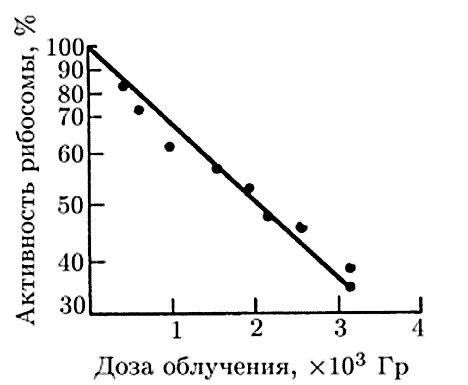
\includegraphics[width=.5\textwidth]{ribosomeInactivation.png}
    \caption{Инактивация лиофилизированных рибосом из клеток \textit{E.coli} $\gamma$-излучением \ce{^{60}Co}.}
    \label{ribosomeInactivation}
\end{figure}
Рибосомы выделяли из клеток E. coli, облучали и инкубировали в системе,
содержащей в качестве мРНК полиуридиновую кислоту (поли-У), которая инициирует
синтез полифенилаланина. Как видно из рисунка, с ростом дозы облучения
экспоненциально снижается доля рибосом, сохранивших исходную синтетическу
активность.

Таким образом, в модельных системах \textit{in vitro} можно анализировать инактивацию нуклеиновых кислот и надмолекулярных комплексов, в которые входят эти макромолекулы. Особых интерес представляют исследования радиационного поражения хроматина. Эти эксперименты приближают нас к пониманию реальных процессов инактивации ДНК в клетке.

Прямое действие радиации на молекулы ДНК, иРНК, тРНК и сложные надмолекулярные ансамбли – рибосомы – приводит к утрате ими биологических функций, связанных с репликацией, транскрипцией и трансляцией генетического кода. Такого рода эффекты имеют решающее значение при действии радиации на вирусы, бактерии, клетки и сложные многоклеточные системы. Поэтому изучению механизмов инактивации нуклеиновых кислот ионизирующим излучением уделяется большое внимание.

\section{Стадии действия ионизирующих излучений на биологические объекты}
% Последовательность событий, происходящих от момента непосредственной
% передачи энергии излучения макромолекуле и до появления в ней стойких
% структурных и функциональных изменений, делится на 3 стадии:
\subsection{Физическая стадия}
На этой стадии энергия излучения переносится веществу, возникают возбужденные и ионизированные молекулы, неравномерно распределенные в объеме вещества. Эти события происходят в первые $10^{-16} - 10^{-13}$ с. 

Для выяснения природы первичных физических процессов необходимо определить параметры «мишени», ответственной за инактивацию молекул. Для решения этой задачи необходим формальный анализ кривых «доза-эффект», сопоставление эффективности излучений с различными ЛПЭ и с различной мощностью дозы, теоретические исследования величин «энергетических пакетов», переносимых молекуле в единичном акте взаимодействия излучения с веществом. Для этой цели привлекаются квантовомеханические представления и сложный математический аппарат. %TODO: Слишком много воды!

\subsubsection{Первичные физические процессы.}
Рассмотрим, выполняются ли условия в случае инактивации белков и
нуклеиновых кислот.

\emph{Первое условие} – экспоненциальный характер кривых «доза– эффект». При облучении сухих или кристаллических белков и нуклеиновых кислот эффект облучения \textit{экспоненциально зависит от поглощенной дозы радиации}. 

\emph{Второе условие} – независимость эффекта, от мощности дозы и от того, ка кими частями она сообщалась объекту, – \textit{также выполняется на различных изученных системах}. 

\begin{wrapfigure}{L}{0.4\textwidth}
    \centering
    \begin{tikzpicture}[scale=.7]
        \begin{axis}[
            ylabel={Ферментативная активность, \%}, 
            ylabel style={
                anchor=south,
            },
            ymode=log,
            xmin=0,
            % xmax=50,
            ymin=1,
            ymax=150,
            xlabel={Доза облучения, $\times 10^5$~Гр}
        ]
        \addplot[black, dashed] {100*e^(-1)} [yshift=12pt] node [pos=0.95] {$D_{37}$};
        \addplot[black, solid,] {100*e^(-(1/1.8)*x)} [yshift=-5pt, xshift=5pt] node [pos=1] {1}; 
        \addplot[black, dashed] coordinates {(1.8, 1) (1.8, 36.787944117)};
        \addplot[black, solid,] {100*e^(-(1/3.2)*x)} [yshift=-5pt, xshift=5pt] node [pos=1] {2};  
        \addplot[black, dashed] coordinates {(3.2, 1) (3.2, 36.787944117)};
        \end{axis}
    \end{tikzpicture}
    \caption{Инактивация трипсина $\gamma$-излучением \ce{^{60}Co}(1) и $\alpha$-частицами поглощения (2) в вакууме}
    \label{inactivationOfTrypsin}
\end{wrapfigure}

О выполнении \emph{третьего условия} – снижения эффективности излучения с ростом ЛПЭ – свидетельствуют многочисленные опыта, результат одного из которых представлен на рисунке \ref{inactivationOfTrypsin}.

Если представление об одноударности процесса инактивации макромолекулы
справедливо, то исходя из величины дозы $D_{37}$, можно определить параметры мишени –
ее геометрические размеры и молекулярную массу.

На основании экспериментально установленных величин $D_{37}$ были рассчитаны
молекулярные массы мишеней, ответственных за инактивацию большого числа
молекул. Во всех случаях, начиная от небольшой молекулы пенициллина, имеющей
молекулярную массу около $10^3$ дальтон\footnote{Единица измерения массы атомов, молекул, а также вирусов, клеток и их структур, равная $1/12$ массы атома углерода (\ce{^{12}C}), или $1,661\cdot 10^{–24}$ грамм}, и до трасформирующей ДНК массой в $10^7$
дальтон, наблюдается хорошее соответствие между молекулярной массой мишени и
истинной молекулярной массой соответствующей молекулы.

\begin{wrapfigure}{R}{0.4\textwidth}
    \centering
    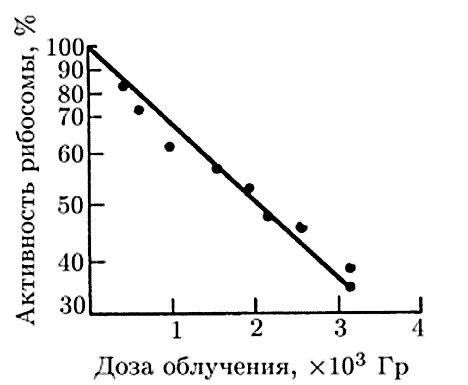
\includegraphics[width=.4\textwidth]{ribosomeInactivation.png}
    \caption{Корреляция между молекулярной массой веществ, определенной физико-химическими методами (М$_\text{физ.-хим.}$) и молекулярной массой мишени, ответственной за инактивацию  (М$_\text{радиац.}$)}
    \label{correlation}
\end{wrapfigure}

Представление о корреляции и этих двух характеристик дает рисунок \ref{correlation}, где по оси абсцисс отложены истинные молекулярные массы веществ, а по оси ординат – молекулярные массы мишеней, ответственные за инактивацию соответствующих молекул. Если характеристики равны по величине, то пересечение проекций их значений в системе координат дает точку, лежащую на прямой, проходящей под углом 45°, как это в действительности и имеет место. 

В большинстве случаев размер мишени близок к геометрическим размерам молекул, т.е. одиночное событие потери энергии в любой точке молекулы приводит к ее инактивации. Этот вывод имеет важное значение. Дальнейший биофизический анализ должен исходить из того факта, что в результате одиночного взаимодействия ионизирующей частицы и молекулы с затратой энергии около 75 эВ молекула белка или нуклеиновой кислоты утрачивает различные функциональные свойства.

Между двумя этими событиями – переносом дискретной порции энергии излучения на макромолекулу и ее инактивацией – происходит ряд последовательных физико-химических процессов, которые требуют детального описания.

\subsubsection{Первичные продукты радиационного превращения молекул}
\begin{wrapfigure}{L}{0.4\textwidth}
    \begin{center}
      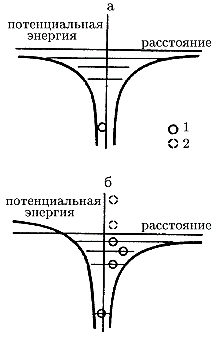
\includegraphics[width=0.4\textwidth]{potentialEnergy.png}
    \end{center}
    \caption{Кривая потенциальной энергии молекулы, взаимодействующей с полем заряженной частицы: a) молекула до наложения поля; б) после взимодействия с полем; 1~---~возбужденная молекула; 2~---~ионизированная молекула}
    \label{potentialEnergy}
\end{wrapfigure}
Передача энергии может происходить за счет двух типов взаимодействия –
лобового и скользящего соударения. Лобовое соударение достаточно точно
описывается классической электродинамикой. При этом типе взаимодействия
осуществляется «прямое попадание» заряженной частицы в орбитальный электрон,
который приобретает необыкновенно большой момент количества движения.
Вероятность этого эффекта низка.

В 8~--~10 раз чаще происходит скользящее соударение, которое служит основным типом взаимодействия заряженной частицы с молекулами.

При описании скользящего соударения частица рассматривается как источник электрического поля, в котором содержатся фотоны всех возможных частот. Такое поле может взаимодействовать с орбитальными электронами на значительных расстояниях. В газах это расстояние («прицельный параметр») порядка 100 нм, в плотном веществе – около 10 нм. Взаимодействие электрического поля заряженной частицы с молекулой переводит ее в то или иное возбужденное состояние, в том числе и соответствующее ионизации (рисунок \ref{potentialEnergy}). 

Силу, с которой электрической поле действует на молекулы, можно разложить на две составляющие: параллельную пути частицы (продольная компонента) и перпендикулярную (поперечная компонента). Каждую компоненту можно изобразить рядом Фурье как сумму чисто гармонических функций времени:
\begin{equation}
    E_\text{попереч.} = \sum k_i \cdot \cos (2\pi\nu_it)
\end{equation}
\emph{«Сила осциллятора»} это характеристика молекулы, взаимодействующей с
заряженной частицей, которая выражает вероятность перехода, приводящего к
возбуждению или ионизации молекулы.

Силу осциллятора, пропорциональную коэффициенту макроскопического
оптического поглощения света, соответствующей частоты, обозначают через $f_s$ для
перехода из основного состояния в дискретное возбужденное состояние $s$, которое
появляется в результате поглощения света частотой $\nu_s = E_s/h$, где $E_s$ – энергия
молекулы в возбужденном состоянии относительно энергии в основном состоянии
(энергия возбуждения). Для переходов внутри непрерывного спектра дискретную силу
осциллятора нужно заменить на $\frac{df}{d\nu}$ или $\frac{df}{dE}$, зависящую от энергии $E = h\nu$. Обе формы выражения силы осциллятора нужно понимать как величины,
усредненные по всем возможным ориентациям молекулы.

Если молекула возбуждается светом источника, дающего равное число фотонов
для каждого интервала частот – от видимого света (белый свет) до рентгеновского
излучения, то число молекул, активированных до состояния $s$, пропорционально силе
осциллятора, этого состояния: $N_s=const \cdot f_s$. Уравнение показывает, что при
постоянном распределении частоты величина $N_s$, пропорциональна силе осциллятора.
Если частота падающего света характеризуется распределением $1/h\nu_s = 1/E_s$, то
число молекул, возбужденных до состояния $s$ прохождением быстрой заряженной
частицы, описывается уравнением $N_s\sim f_s/E_s$. Аналогичное выражение для
непрерывного спектра: 
\begin{equation}
    N(E)\sim \left (\frac{df}{E} \right )\frac{1}{E}. 
\end{equation}
Уравнение называют \emph{«оптическим приближением»}. Основное ограничение этого метода – значительная погрешность при малых значениях $f_s$. Однако применение оптического приближения дает хорошие результаты для анализа энергетического спектра первичных активаций, генерируемых
излучением, в действующем спектре которого преобладают быстрые заряженные частицы.

Сила осциллятора $f_s$ пропорциональна числу электронов в оболочке, в которой
индуцируется активация, т.е. она максимальна для внешних оболочек; $E_s$,
пропорциональна квадрату эффективного заряда ядра и менее значима, для внешних
оболочек, так как электроны внутренних оболочек экранируют поле ядра. Поэтому,
согласно уравнениям, можно сделать вывод: \textbf{активация валентных электронов – преобладающий первичный процесс, происходящий в результате прохождения
заряженной частицы через вещество}.

Анализ спектра возбуждения молекул, состоящих из атомов с $Z < 10$ и поэтому
имеющих кроме валентных электронов только К- оболочку, показал, что практически
все возбуждения сосредоточены в области сравнительно больших значений $Е$.
Непрерывный спектр поглощения молекул, в котором сосредоточена сила
осциллятора, содержит в себе непрерывные спектры, обусловленные процессом
ионизации и процессом диссоциации, а также спектр, создаваемый процессами, в
которые возможна как ионизация, так и диссоциация молекулы, конкурирующие
между собой (сверхвозбужденное состояние).

\begin{wrapfigure}{R}{0.5\textwidth}
    \begin{center}
      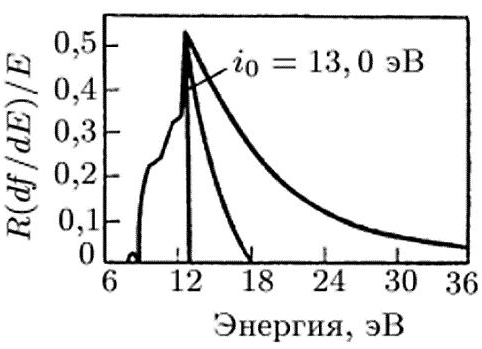
\includegraphics[width=0.5\textwidth]{methanSpectrum.png}
    \end{center}
    \caption{Спектр возбуждения метана}
    \label{methanSpectrum}
\end{wrapfigure}

На рисунке \ref{methanSpectrum} показан спектр возбуждения метана, построенный на основании экспериментальной оценки силы осциллятора молекулы. Видно, что из всех первичных событий, которые не приводят к ионизации, 45\% составляют сверхвозбужденные состояния. Среднее значение энергии, соответствующее полосе сверхвозбуждения, равно приблизительно 15 эВ, т.е. более чем в 3 раза превосходит энергию диссоциации $CH_3-H$, равную 4,4 эВ. В этом сверхвозбужденном состоянии существует конкуренция между явлениями ионизации и диссоциации. Часть спектра, обозначенная как «ионизация», соответствует тем уровням возбуждения, которые всегда приводят к ионизации.

Анализ спектров возбуждения показывает, что для большинства, органических
молекул спектр сил осцилляторов лежит в области примерно 10~--~30 эВ над основным
состоянием. Сила более длинноволновых осцилляторов невелика (исключение
составляют молекулы, имеющие двойные и тройные связи: они могут возбуждаться и
при меньших энергиях).В большинстве случаев спектры энергий осцилляторов превышают потенциал
ионизации. Однако не все состояния с энергиями, превосходящими потенциал
ионизации, непременно приводят к ионизации молекулы. \textit{«Сверхвозбужденные
состояния» могут рассеивать энергию при внутримолекулярных изменениях или при
диссоциации молекулы на два радикала}.

Только часть спектра, обозначаемая как «ионизация», относится к тем
переходам, которые всегда, приводят к потере электрона.

Величину «пакетов энергии», передаваемых макромолекуле в результате
одиночного взаимодействия, можно получить путем прямого измерения потери
энергии электронами, проходящими через тонкие пленки, для которых вероятность
более чем одного взаимодействия с электроном крайне мала.
\begin{figure}[htbp]
    \centering
    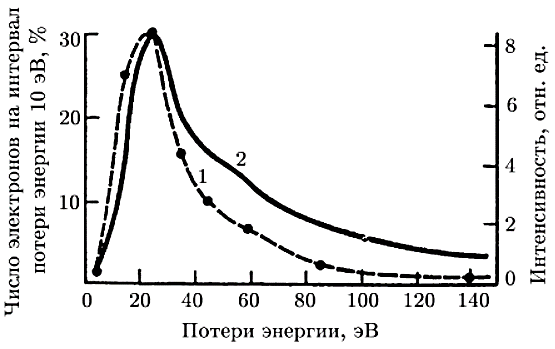
\includegraphics[width=.6\textwidth]{energyLosses.png}
    \caption{Распределение потери энергии электронами, проходящими через тонкие слои органического вещества: 1 — электроны 20 кэВ проходят через слой полимера «формвар» толщиной 130~\AA; 2 — электроны с энергией 150 кэВ проходят через пленку ДНК толщиной 2000~\AA}
    \label{energyLosses}
\end{figure}
Данные 1 на рисунке \ref{energyLosses} можно рассматривать как меру распределения частоты
различных событий потери энергии. Из рисунка видно, что чрезвычайно редко
величина потери энергии меньше 10 эВ. С наибольшей частотой при каждом
первичном взаимодействии переносится пакет энергии в 22 эВ, в то время как среднее
количество потери энергии на одно событие взаимодействия 60 эВ.
Спектры потери энергии в формваре и ДНК качественно сходны. Различие,
вероятно, связано с неодинаковой толщиной пленок. При такой толщине слоя ДНК
можно ожидать более одного события потери энергии. Следует также учесть, что оба
рассматриваемых спектра включают и небольшое число лобовых соударений. Если сделать необходимые поправки на эти эффекты, то мы получим спектр возбуждения
ДНК, который позволил бы оценить спектр сил осцилляторов этой молекулы.

\subsubsection{Вывод}
Итак, прямые эксперименты показывают, что на одно событие потери энергии в
среднем на макромолекулы переносится 60 эВ энергии излучения. Эта величина
значительно превосходит потенциал ионизации молекулы. Перенос такого большого
количества энергии с высокой вероятностью переводит молекулу в ионизированное
состояние. Помимо ионизированных, возникают возбужденные и сверхвозбужденные
молекулы.

Относительный вклад ионизации и возбуждения в биологический эффект можно
оценить некоторыми специальными методами.

Возбуждение различных осцилляторов приводит к появлению возбужденных,
сверхвозбужденных и ионизированных молекул.
%  Теоретический расчет выхода этих
% первичных продуктов требует знания действующего спектра, сечения возбуждения и
% ионизации и представляет пока еще не решенную задачу. 
Метод \emph{«оптического приближения»} позволяет оценить соотношение этих продуктов исходя из
распределения спектра сил осциллятора молекулы. Информацию о распределении
силы осциллятора молекулы можно получить на основании косвенных экспериментов
с использованием различных физических методов.

Первая, или физическая, стадия действия излучения заканчивается образованием первичных продуктов, т.е. возбужденных, сверхвозбужденных и ионизированных молекул, неравномерно распределенных в пространстве.

Прямые эксперименты показывают, что на одно событие потери энергии в среднем на макромолекулы переносится 60 эВ энергии
излучения. Эта величина значительно превосх0дит потенциал иониза-
ции молекулы. Перенос такого большого количества энергии с высокой
вероятностью переведит молекулу в ионизированное состояние. Поми—
мо ионизированных, возникают возбужденные и сверхвозбужденные
молекулы.

\subsection{Физико-химическая стадия}
Состоит из различных типов реакций, приводящих к перераспределению между
возбужденными молекулами избыточной энергии.
\[ t = 10^{-12} - 10^{-10}\;c\]
Облученные молекулы, находящиеся в различных электронно-возбужденных
состояниях, в течение физико- химической стадии имеют много возможностей для
дальнейших превращений. В результате появляются разнообразные активные
продукты: ионы, радикалы. Поэтому в веществе, состоящем даже из одного типа
молекул, облучение генерирует ионы и радикалы с широким спектром химических
свойств.

Для изучения этой стадии исследуют спектр первичных продуктов, возникающих в результате физико-химических процессов перераспределения избыточной энергии, поглощенной молекулами. Особая роль здесь принадлежит методу электронного парамагнитного резонанса (ЭПР) и другим способам идентификации свободных радикалов.

На рисунке \ref{timeScale} представлена временная шкала различных процессов, в результате
которых молекула перераспределяет избыточную энергию или избавляется от нее.
\begin{figure}[htbp]
    \centering
    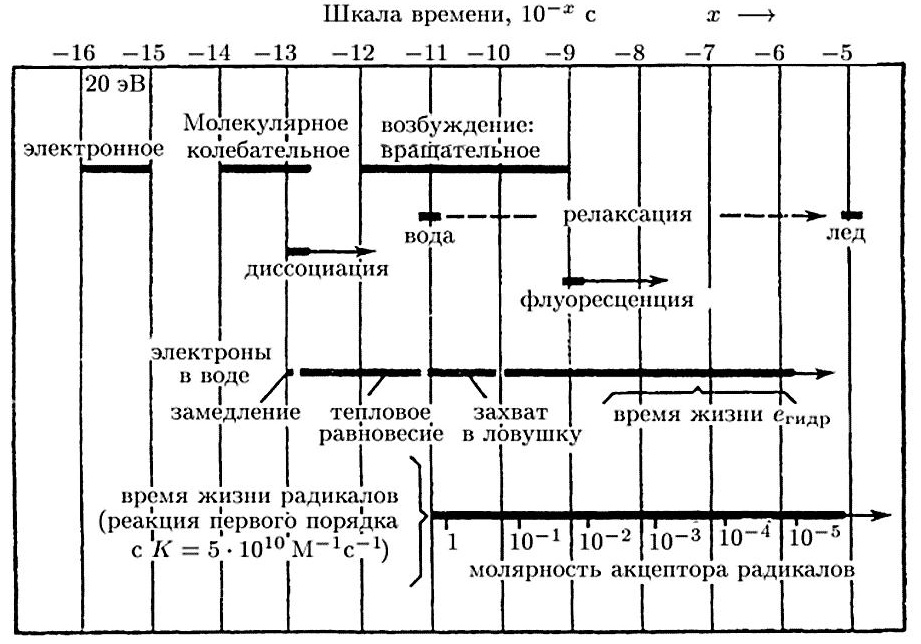
\includegraphics[width=\textwidth]{timeScale.jpg}
    \caption{Временная шкала процесса превращений энергии, передаваемой заряженными частицами молекулам среды}
    \label{timeScale}
\end{figure}
Нижний предел времени, необходимый для передачи энергии от частицы к
частице, устанавливается принципом неопределенности Гейзенберга. Передача
энергии E, сравнимой с энергией связи электрона в молекуле, требует времени,
равного по порядку величины периоду колебаний электрона – $10^{16}-10^{15}$ с. Этого
времени достаточно для любой перестройки электронной системы сильно
возбужденной молекулы. Однако на самом деле некоторые из сильно возбужденных
состояний существуют в сотни раз дольше. Это означает, что с процессами ионизации могут конкурировать процессы внутренней перестройки, сопровождающиеся
смещением атомов в молекулах.

\emph{Сверхвозбужденные молекулы} – это молекулы, обладающие избыточной
энергией, которая превышает потенциал ионизации. Существуют экспериментальные
данные, подтверждающие представления о том, что сверхвозбужденное состояние в
сложных молекулах сохраняется в течение времени, примерно в 100 раз
превышающего период колебаний, т.е. больше $10^{-13}$ с. Некоторые из
сверхвозбужденных состояний возникают в результате одновременного перехода двух
или нескольких электронов на более высокие энергетические уровни. Взаимодействие
таких уровней может привести к концентрации энергии в одном из электронов. Если
этот эффект произойдет, то электрон будет выброшен из молекулы, а сама она станет
положительным ионом. С такой «автоионизацией» конкурируют процессы внутренней
перестройки молекулы, в том числе и те, которые приводят к смещению атомов и
переходу избыточной энергии в химическую и тепловую, что ведет к уменьшению
имеющейся энергии до значений, меньших порога ионизации. Таким образом, в
сверхвозбужденных молекулах существует конкуренция между процессом ионизации
и диссоциации.

\emph{Ионизацию} можно рассматривать как одну из форм возбуждения, при которой
электрон или группа электронов приобретает настолько большой запас энергии, что
выбрасывается из молекулы. Образуются ионы, находящиеся в состоянии
электронного и, как правило, некоторого колебательного возбуждения. Это
происходит потому, что межатомные расстояния в ионе, находящемся в основном
состоянии, и в нейтральной молекуле различаются между собой, акт же ионизации
происходит значительно быстрее перестройки связи (принцип Франка-Кондона). В
результате ион начинает свое существование с атомными расстояниями,
отличающимися от нормальных и соответствующими некоторой колебательной
потенциальной энергии. Процесс внутренней конверсии, рассмотренный выше для
возбужденных молекул, происходит аналогичным образом и в ионе, если ион
изолирован; концентрация колебательной энергии на определенных связях может
привести к его распаду. В жидкостях и твердых телах быстрое рассеяние колебательной энергии в состоянии предотвратить распад и позволить иону перейти в
низшее электронное состояние, в котором он способен существовать некоторое время.
Если затем ион встретится с каким-либо отрицательно заряженным образованием
(ион, сольватированный электрон и т.д.), энергия соединения может оказаться
достаточной для распада молекулы на два свободных радикала.

Таким образом, дальнейшие превращения, которые испытывает ионизированная
молекула, вероятнее всего приведут ее к распаду на два свободных радикала.

\subsubsection{Судьба электронов}
Электроны, выбитые из молекулы, обычно делят на две группы в соответствии с
тем, больше их кинетическая энергия энергии низшего уровня электронного
возбуждения молекул окружающей среды или меньше ее. Электроны первой группы
взаимодействуют с электронной системой молекул, с которыми они сталкиваются, и
теряют энергию в неупругих соударениях. В конце концов они переходят во вторую
группу, оставляя на своем пути ряд молекул с электронными возбуждениями. В
дальнейшем эти электроны теряют энергию за счет возбуждения колебательных и
вращательных движений в сталкивающихся с ними молекулах.

Если в среде преобладают молекулы, у которых энергия низшего уровня
электронного возбуждения существенно превышает кинетическую энергию электрона,
но в этой же среде имеется небольшая доля молекул с низкими энергиями
электронного возбуждения, то электроны, теряющие мало энергии при столкновении с
молекулами первого типа, будут «разыскивать» и возбуждать молекулы второго типа,
передавая значительно большую часть поглощенной энергии, чем это соответствовало
бы их малой концентрации в среде. По данным Платцмана 15~--~20\% всей энергии,
поглощенной при воздействии высокоэнергетического излучения, передается
медленными электронами, и среднее время, необходимое для достижения ими
теплового равновесия со средой, составляет примерно $10^{-11}$ с. За время такого же
порядка происходит поляризация среды вокруг замедлившегося электрона. Возникает
чрезвычайно активное в химическом отношении образование, названноесольватированным электроном (в водной среде это так называемый \emph{«гидратированный электрон»}, о котором подробнее сказано в
 следующей главе). %TODO: добавить раздел

\subsubsection{Вывод}
Процессы, происходящие на физико-химической стадии, приводят к различным
типам перераспределения возбужденными молекулами избыточной энергии и, таким
образом, обусловливают появление разнообразных активных продуктов (ионов,
радикалов и т.д.). Эти процессы протекают в течение очень короткого интервала
времени, порядка $10^{-12}-10^{-10}$ с.

\subsection{Химическая стадия}
На этой стадии ионы и радикалы взаимодействуют друг с другом и с окружающими молекулами, формируя структурные повреждения различного типа.
\[ t = 10^{-6} - 10^{-3}\;c\]
Для выявления разного типа структурных повреждений молекул используется
современный арсенал физических и химических методов анализа макромолекул.

\subsubsection{Структурные повреждения, возникающие в облученных
макромолекулах}
Важнейший этап биофизического анализа инактивации молекул ИИ состоит в
структурных типах повреждения молекул, выяснения природы процессов,
приводящих к данному типу повреждений.

Анализ структурных повреждений, возникающих в облученной макромолекуле,
представляет собой сложную экспериментальную задачу, требующую использование
высокочувствительных методов исследования.

Структурные повреждения, выявляемые в облученных нуклеиновых кислотах.

При облучении сухих препаратов ДНК, возникает ряд повреждений, которые
удается количественно оценить при использовании высоких доз облучения порядка 10~Гр. Это превосходит значение дозы $D_{37}$.

Для выявления структурных повреждений нуклеиновых кислот,
сопровождающихся изменением их размеров, используют различные методы
измерения молекулярной массы препарата, т.к. молекулярная масса изменяется
вследствие разрыва полимерной цепи.

Влияние облучения на состояние систем водородных связей в молекуле ДНК,
оценивают по возникновению в ней участков денатурации.

Использование различных методов позволило установить, что в результате облучения сухих препаратов ДНК возникают следующие типы структурных
повреждений макромолекул:
\begin{enumerate}
    \item однонитевые и двунитевые разрывы;
    \item межмолекулярные поперечные сшивки полинуклеотидных цепей;
    \item разветвленные цепи вследствие суммарного эффекта, которые образуются за счет присоединения обломков молекулы, образованной в результате двунитевого
    разрыва, к местам однонитевых разрывов в цепях.
\end{enumerate}
Эксперименты показывают, что все разрывы пропорциональны поглощенной
дозе излучения. Это означает, что разрывы вызываются событиями поглощения
энергии ионизирующим излучением.

\subsubsection{Структурные повреждения облученных ферментов}
Большинство исследований по радиационной химии протеинов выполнено на
белках с известной первичной структурой.
Анализ структурных повреждений, возникающих в облученных препаратах
рибонуклеазы, показал, что при дозах, близких к $D_{37}$, наблюдается:
\begin{itemize}
    \item изменение аминокислотного состава; заметнее всего в образцах снижалось
    содержание 6 аминокислот: метионина, фенилаланина, лизина, гистидина, тирозина и
    цистина;
   \item нарушение третичной структуры макромолекулы, оцениваемое но изменению
    оптического поглощения и оптического вращения, доступности остатков тирозина,
    степени переваривания белка трипсином и т.д.;
   \item возникновение разрывов полипептидной цепи, приводящее к появлению
    свободных амидных групп и фрагментов молекулы;
   \item появление агрегатов, о наличии которых судили по изменению константы
    седиментации и скорости элюции при хроматографии на колонках из сефадекса;
   \item разрыв сульфгидрильных связей и появление свободных SН-групп.
\end{itemize}
При облучении \emph{лизоцима} обнаружен несколько иной характер структурных повреждений:
\begin{itemize}
   \item изменяется конформация макромолекулы;
   \item появляется несколько компонентов, обладающих ферментной активностью;
   \item не обнаруживаются изменения в аминокислотном составе макромолекулы.
\end{itemize}
Исследование структурных повреждений облученного \emph{химотрипсина} показало,
что поглощение энергии ионизирующих излучений вызывает:
\begin{itemize}
    \item появление новых хроматографических пиков при элюции облученного
    препарала; эти фрагменты утратили ферментную активность;
   \item возникновение конформационных изменений, выявляемых по изменению
    оптического вращения и уменьшению прочносвязанных амидных атомов водорода;
   \item разрушение аминокислотных остатков серина и триптофана (в среднем одна
    молекула серина и одна триптофана на молекулу фермента при дозе D37); %TODO: привести 37 к индексу
   \item снижение способности активного центра фермента связывать субстрат.
\end{itemize}
При облучении лизоцина обнаружен иной характер структурных повреждений.
Изменяется конформация макромолекул, появляются несколько компонентов,
обладающих ферментативной активностью, изменений в аминокислотном составе макромолекулы не обнаружены.

В диапазоне больших доз радиации, картина существенно усложняется за счет
возникновения повторных актов взаимодействия, вызывающих дополнительные
повреждения.
\begin{figure}[htbp]
    \centering
    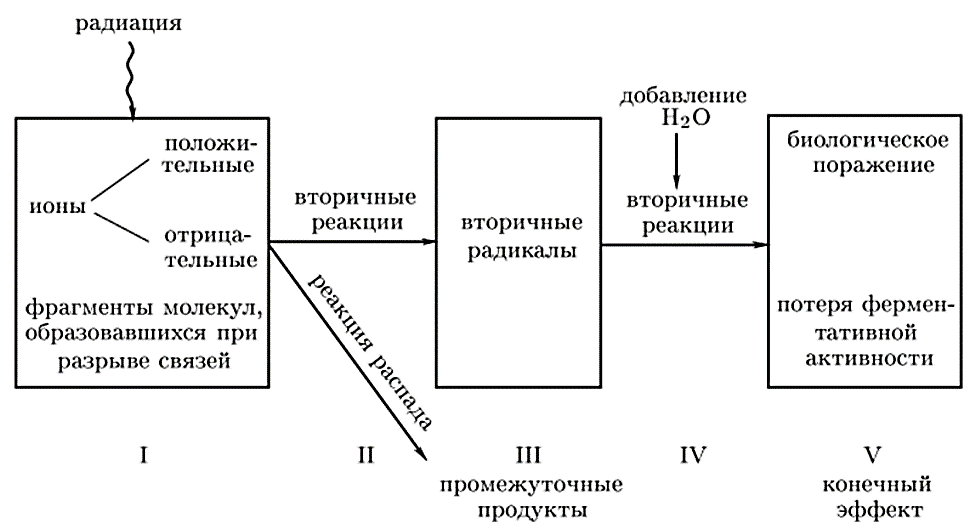
\includegraphics[width=\textwidth]{radInacModel.png}
    \caption{Свободнорадикальная модель радиационной инактивации сухих ферментов: I — спектр первичных продуктов; II — процессы, протекающие на физико-химической стадии; III — образовавшиеся промежуточные продукты; IV, V — конечный эффект — инактивации фермента}
    \label{radInacModel}
\end{figure}

\section{Миграция энергии излучения в биологических структурах}
Анализ кривых «доза-эффект» свидетельствует о том, что инактивация фермента
может произойти в результате одиночного события потери энергии излучения в любой
точке макромолекулы (параметры мишени совпадают с истинными размерами
макромолекулы). Представление об одноударности процесса инактивации означает,
что поглощение энергии в любой точке молекулы однозначно приводит к изменению
ее биологических свойств. Однако при объяснении механизма инактивации фермента
в результате одиночного события попадания следует иметь в виду, что определенный
тип инактивации (например, утрата субстратной специфичности) может быть связан
со структурным повреждением, возникшим не в любом, а, скорее всего, в
определенном участке макромолекулы.

Теоретический анализ спектра сил осцилляторов молекулы и результаты прямых
измерений потери энергии, приходящейся на одно взаимодействие, показывают, что
ускоренные заряженные частицы с большой вероятностью переносят к макромолекуле
значительные порции энергии, в среднем около 60 эВ. Этого более чем достаточно для
разрыва любой химической связи и удаления электрона из молекулы.

\textit{Существует ряд прямых способов доказательства миграции энергии
возбуждения внутри молекулы и между молекулами.}

\emph{Термолюминесценция} возникает как следствие рекомбинации (по мере
повышения температуры) короткоживущих продуктов, «замороженных» при
температуре жидкого азота. Повышение температуры приводит к увеличению
подвижности первичных продуктов (короткоживущих радикалов, электронов), что
способствует реакциям их друг с другом и образованию вторичных продуктов. В
процессе этих реакций и регистрируется термолюминесценция.

\emph{Измерение сигнала ЭПР}. Для исследуемого радикала возникает характерный сигнал ЭПР  в результате взаимодействия магнитного момента,
неспаренного электрона с магнитными полями окружающих ядер и электронов, т.е.
сигнал ЭПР изменяется в зависимости от локализации неспаренного электрона.

\emph{Реакция присоединения.} Существование этого типа реакций прямо указывает на возможность переноса энергии от облученных белков к низкомолекулярным молекулам-примесям. Перенесенная энергия расходуется на отрыв от молекулыпримеси «$H-M$» атома водорода, который присоединяется к радикалу белка:
\[ R' + HM \rightarrow RH + M'\]
Еще один возможный механизм переноса энергии – это \emph{миграция электронов
через зону проводимости с последующим захватом их положительно
заряженными «дырками»}.

Перенос энергии возбуждения и перенос электронов требуют участия
специальных структур и, возможно, высоких энергий активации, тогда как
экспериментально наблюдаемые значения энергии активации радикалообразования и
инактивации различных молекул довольно малы. Эти факты позволяют предположить,
что именно перенос радикалов имеет большое значение в процессах миграции энергии
при прямом действии радиации.

\section{Модификация лучевого поражения макромолекул}
Чувствительность макромолекул к радиационному воздействию можно изменить по меньшей мере в два или три раза в зависимости от условий во время облучения или после него. 

К числу агентов, которые модифицируют радиочувствительность макромолекул, относятся \emph{кислород, температурное воздействие, присутствие молекул-примесей} и др. 

Каждый из этих факторов, естественно, не может повлиять на физический акт переноса энергии излучения к макромолекуле, и все-таки эти воздействия способны усилить или ослабить лучевое повреждение. Поэтому считают, что модифицирующие агенты влияют не на первичные акты абсорбции энергии, а на более поздние этапы лучевого поражения.

Например, они могут изменить характер миграции энергии внутри макромолекулы или между молекулами, избирательно защитить определенные функциональные группы, репарировать лучевые повреждения или изменить характер физико-химических реакций, в которые вступают облученные молекулы.

\subsection{Модифицирующее действие кислорода}
В экспериментах с сухими препаратами ферментов было установлено, что их радиочувствительность значительно возрастает, если облучение проводится в атмосфере кислорода, а не в вакууме. 

На рисунке \ref{inactivationWithOxigen} представлены результаты эксперимента по сопоставлению эффективности инактивации сухой РНКазы ɣ-излучением в вакууме и в атмосфере кислорода. Значение дозы D37 для инактивации рибонуклеазы в вакууме примерно вдвое выше, чем в атмосфере $O_2$.
\begin{figure}[htbp]
    \begin{minipage}{.48\textwidth}
        \centering
        \begin{tikzpicture}[scale=.7]
            \begin{axis}[
                ylabel={Ферментативная активность, \%}, 
                ylabel style={
                    anchor=south,
                },
                ymode=log,
                xmin=0,
                % xmax=50,
                ymin=5,
                ymax=150,
                xlabel={Доза облучения, $\times 100$~Гр}
            ]
            \addplot[red, solid,] {100*e^(-(1/2)*x)} [yshift=-8pt, xshift=-5pt] node [pos=0.7] {2} [anchor=east] node [pos=0.85] {$D_{37} = 200$ КГр}; 
            \addplot[green, solid,] {100*e^(-(1/4.2)*x)} [yshift=-8pt, xshift=-5pt] node [pos=0.8] {1} [yshift=2pt, anchor=south west] node [pos=0.7] {$D_{37} = 420$ КГр};  
            \end{axis}
        \end{tikzpicture}
        \caption{Инактивацня сухой РНКазы $\gamma$-излучением \ce{^{60}Co} в вакууме (1) и в присутствии кислорода (2)}
        \label{inactivationWithOxigen} 
    \end{minipage} \hfill
    \begin{minipage}{.48\textwidth}
        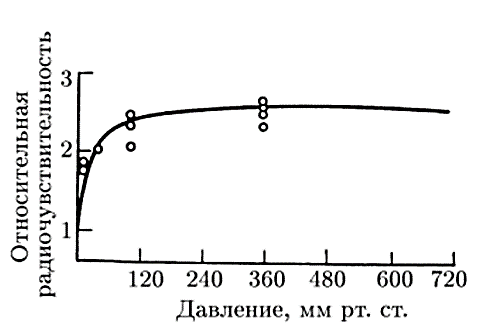
\includegraphics[width=\textwidth]{trypsinDependsOnOxygen.png}
        \caption{Относительная чувствительность сухого трипсииа к действию $\gamma$-излучеиия в зависимости от содержания кислорода во время облучения (за единицу принята радиочувствительность трипсина в вакууме)}
        \label{trypsinDependsOnOxygen} 
    \end{minipage}
    
\end{figure}

На рисунке \ref{trypsinDependsOnOxygen} видно, что даже незначительное содержание кислорода в среде приводит к резкому возрастанию инактивирующего действия данной дозы облучения. При увеличении давления $O_2$ примерно до 120 мм рт. ст. эффект инактивации возрастает, дальнейшее повышение содержания кислорода в среде оказывается неэффективным.

\emph{Кислородное последействие}~---~пострадиационное действие кислорода на
ферменты, после изучения которого было показано, что при облучении ферментная
активность не теряется и в анаэробных условиях может сохраняться длительное время.
В отсутствие воды кислород также не оказывал инактивирующего действия, и лишь при увлажнении препарата происходила его инактивация под действием кислорода,
степень которой увеличивалась с ростом поглощенной дозы.

Отсутствие поражения некоторых объектов при анаэробном облучении
свидетельствует, что кислород не просто один из агентов, модифицирующих
поражение, а необходимый участник определенных видов поражения. При этом
кислород может оказать поражающее действие, присутствуя не только во время
облучения, но и после его окончания.

\subsection{Влияние температуры во время прямого действия радиации}
Радиочувствительность многих макромолекул зависит от температуры во время облучения. Пример этого приведен на рисунке \ref{inactivationOfRNAWithVariousTemp}, где показана инактивация сухой РНКазы $\gamma$-излучением при трех различных температурах.  

\begin{wrapfigure}{L}{0.4\textwidth}
    \centering
    \begin{tikzpicture}[scale=.7]
        \begin{axis}[
            ylabel={Ферментативная активность, \%}, 
            ylabel style={
                anchor=south,
            },
            ymode=log,
            xmin=0,
            % xmax=50,
            ymin=10,
            ymax=150,
            xlabel={Доза облучения, $\times 10^5$~Гр}
        ]
        \addplot[black, dashed] {100*e^(-1)} [yshift=-12pt, anchor=west] node [pos=0.6] {$D_{37}$};
        \addplot[black, solid,] {100} [yshift=-10pt, anchor=east] node [pos=.95] {71 K}; 
        \addplot[black, solid,] {100*e^(-(1/10)*x)} [yshift=-5pt, anchor=east] node [pos=.95] {195 K};  
        \addplot[black, solid,] {100*e^(-(1/4)*x)} [yshift=-5pt, anchor=east] node [pos=.95] {310 K};  
        \end{axis}
    \end{tikzpicture}
    \caption{Инактивацня РНКазы $\gamma$-излучением \ce{^{60}Co} в вакууме при различных температурах}
    \label{inactivationOfRNAWithVariousTemp}
\end{wrapfigure}

Механизм температурного эффекта также окончательно еще не установлен. Предполагают, что константа скорости реакции (или реакций), определяющей инактивацию макромолекулы, зависит от повышения температуры. По крайней мере некоторыми из таких реакций могут быть взаимодействия макромолекул с атомарным водородом и другими малыми радикалами, которые высвобождаются при облучении органических материалов и, вероятно, атакуют непораженные молекулы. 

Температурное последействие. В облученных белковых молекулах возникают скрытые повреждения, переходящие в явные при дополнительном тепловом воздействии. Например, возникающие внутримолекулярные повреждения приводят к инактивации фермента после обработки облученного препарата, теплом. Тепловое воздействие эффективно и после аэробного облучения, т.е. в результате нагрева, реализуются иные скрытые повреждения, чем те, на которые способен воздействовать
кислород. Таким образом, в одной и той же макромолекуле могут возникать по
крайней мере два типа скрытых повреждений: независимые от кислорода и зависимые
от присутствия его. В то же время под влиянием тепла не могут быть реализованы все
типы скрытых повреждений.

Природа скрытых повреждений, требующих для своей реализации
дополнительного теплового воздействия, продолжает исследоваться в настоящее
время.

\subsection{Роль примесей}
Облучение белков в смеси с рядом низкомолекулярных веществ может
уменьшить радиочувствительность (эффект защиты) или увеличить ее
(сенсибилизация).

Защитным действием обладают тиолы и индолилалкинамины – классические
радиопротекторы.

Существуют и вещества, усиливающие радиочувствительность (сахароза).
Защитное действие может осуществляться за счет высокой конкуренции за
высокоактивные свободные радикалы, которые могут вызывать структурные
повреждения.

Другая возможность в том, что агент способствует восстановлению
повреждений молекулы. Модифицирующее действие низкомолекулярных примесей
используют для выяснения роли миграции энергии при радиобиологических
процессах. Использование агентов является традиционным приемом биохимического
анализа.

\section{Непрямое действие излучения. Радиолиз воды. Радиационно-химические
превращения молекул воды. Гидратированный электрон}
% Общая характеристика непрямого действия ионизирующих излучений на
% макромолекулы в водных растворах
Если облучению подвергаются водные растворы в низкой концентрации, в
которых каждую биомакромолекулу окружает множество молекул воды, товероятность поглощения энергии ионизирующего излучения водой или органической
молекулой примерно одинакова. Поэтому в разбавленных водных растворах большая
часть энергии будет поглощаться молекулами воды, которых значительно больше, чем
растворенных биомакромолекул.

Если в результате поглощения энергии ионизирующего излучения вода
становится «химически активной», то растворенные молекулы будут испытывать
дополнительное поражение.

\begin{wrapfigure}{L}{0.4\textwidth}
    \centering
    \begin{tikzpicture}[scale=.7]
        \begin{axis}[
            ylabel={Ферментативная активность, \%}, 
            ylabel style={
                anchor=south,
            },
            ymode=log,
            xmin=0,
            xmax=12,
            ymin=10,
            ymax=150,
            xlabel={Доза облучения, $\times 10^4$~Гр}
        ]
        \addplot[black, dashed, domain=0:12] {100*e^(-1)} [yshift=-12pt, anchor=west] node [pos=0.6] {$D_{37}$};
        \addplot[green, solid, domain=0:12] {100*e^(-(1/42)*x)} [yshift=-8pt, anchor=east] node [pos=.95] {1};  
        \addplot[red, solid,] {100*e^(-2.5*x)} [anchor=south west] node [pos=.57] {2};  
        \end{axis}
    \end{tikzpicture}
    \caption{Инактивацня РНКазы $\gamma$-излучением \ce{^{60}Co} в сухом состоянии (1) и в водном растворе фермента в конценрации 5 мг/мл (2)}
    \label{inactivationOfWetAndDryRNA}
\end{wrapfigure}
На рисунке \ref{inactivationOfWetAndDryRNA} сопоставлена радиочувствительность рибонуклеазы в сухих препаратах и в водном растворе. Как следует из данных эксперимента, если значение дозы D37 для инактивации сухого фермента составляет 420 кГр, то в водном растворе сравнимая инактивация достигается после облучения в дозе 4 кГр. 

Такой результат характерен для различных макромолекул – белков, нуклеиновых кислот, и др.; в разбавленном водном растворе их радиочувствительность возрастает в десятки и сотни раз.

Зависимость «доза-эффект» при облучении водных растворов макромолекул
носит экспоненциальный характер, аналогично наблюдаемому при облучении сухих
препаратов. Это указывает на одноударность процесса инактивации. При однодарном
механизме объем мишени, ответственной за инактивацию, пропорционален $1/D_{37}$.

Для рассматриваемого случая поражения мишеней, растворенных в воде,
вводится понятие \emph{«эффективного объема»}, или такого объема, из любого места
которого энергия попадания, не растраченная до уровня, более низкого, чем порог
действия, тем или иным путем достигнет «места действия» (например, определенного
структурного звена, макромолекулы, ответственного за инактивацию) и приведет к
возникновению «единицы реакции» (т.е. к инактивации фермента). В водном растворе энергия, поглощенная растворителем, может передаваться растворенной
макромолекуле за счет диффузии активных продуктов радиолиза воды.

Для сравнения энергий активации необходимо определять величину
радиационно-химического выхода G инактивации фермента, в растворе и в сухом
препарате из соотношения:
\begin{equation}
    G = \frac{\text{число образованных или пораженных молекул}}{\text{100 эВ поглощённой энергии}}
\end{equation}
В опытах с РНКазой установлено, что $G$ в сухом препарате равна 1,68, в водном
растворе – 0,89. Обе величины относительно мало отличаются друг от друга.

Мы можем говорить об увеличении эффективности данной дозы, которое
обусловлено увеличением объема чувствительной мишени. В мишень большего
размера более вероятно одиночное попадание, приводящее к инактивации.

Для изучения механизма радиационной инактивации растворенных в воде
молекул необходимо осуществить ряд логически связанных друг с другом этапов
биофизического анализа:
\begin{itemize}
    \item изучить характер радиационно-химического превращения молекул воды,
    природу возникающих активных продуктов, их физико-химические свойства и
    реакционную способность;
    \item  установить кинетические характеристики процесса инактивации растворенных
    молекул;
    \item  определить основные типы реакций, в которые могут вступать органические
    молекулы и продукты радиолиза воды;
    \item  исследовать характер структурных повреждений, возникающих в
    биомакромолекулах, взаимодействующих с активными продуктами радиолиза воды, и
    найти причинно-следственную связь между типами структурного повреждения и
    характером инактивации растворенных макромолекул.
\end{itemize}
Рассмотрим ряд методических подходов к решению перечисленных задач и биофизических исследованиях.

% Биофизический анализ радиационной инактивации молекул в растворах
\subsection{Радиационно-химические превращения молекул воды.}
\begin{wrapfigure}{L}{0.4\textwidth}
    \centering
    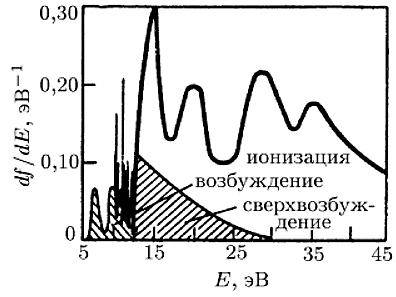
\includegraphics[width=.4\textwidth]{spectrumOfWater.png}
    \caption{Оптический спектр поглощения воды}
    \label{spectrumOfWater}
\end{wrapfigure}
На рисунке \ref{spectrumOfWater} представлен оптический спектр поглощения воды, дающий представление о распределении сил осцилляторов молекулы $H_2O$. 

В части спектра, соответствующей обычному возбуждению с энергией, меньшей потенциала ионизации I = 12,6 эВ, можно различить три области. Полоса непрерывного поглощения с наименьшей энергией обусловлена только переходом, который приводит к диссоциации с образованием основного (электронного) состояния $H + OH$ и ответственен за известную непрозрачность воды во всех фазовых состояниях для длин волн короче 180 нм. В другие полосы возбуждения входят как область непрерывного поглощения, так и ряд отчетливых полос, в которых соответствующие им наиболее распространенные первичные продукты диссоциируют на H и OH* или $H_2$ и $O$. 

Область сверхвозбуждения простирается от $I_0$ до энергии около 30 эВ. Сверхвозбуждение возникает в результате примерно 63\% всех первичных событий, происходящих без ионизации, а конкуренция между двумя путями – ионизацией и диссоциацией – была доказана экспериментально. 

До середины 60-х гг. считалось, что при облучении водных растворов макромолекул косвенное поражение их происходит за счет взаимодействия с радикалами $Н'$, $ОН'$ и перекисью водорода. 

Дальнейшие исследования привели к открытию в облученной воде особой стабилизированной формы электрона, которая получила, название \emph{«гидратированный электрон»}.

\begin{wrapfigure}{R}{0.4\textwidth}
    \centering
    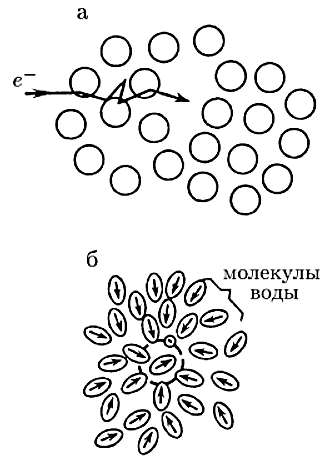
\includegraphics[width=.4\textwidth]{hydratedElectron.png}
    \caption{Гидратированный электрон: а) схематическое представление последнего участка пути «свободного электрона» в жидкости; б) основная ориентация полярных молекул воды вокруг гидратированного электрона}
    \label{hydratedElectron}
\end{wrapfigure}
Гидратированный электрон, обозначаемый \emph{\ce{e^{-}_{гидр.}}}, возникает в результате
стабилизации свободного электрона в «потенциальной яме», образованной
поляризованными молекулами воды (рис. \ref{hydratedElectron} а, б).

Растеряв на возбуждение и ионизацию среды большую часть энергии, электрон
продолжает взаимодействовать с окружающими его молекулами до тех пор, пока
он в конце концов не окажется в «потенциальной яме», так как не сможет
преодолеть электростатическое отталкивание электронного облака молекулы, через которую
он проходит.

Гидратированный электрон, который в химическом отношении ведет себя, как очень
активный ион, вступая в реакции со многими веществами при первом соударении. Скорость
реакции ограничена временем, необходимым для того, чтобы перемещающиеся в результате диффузии реагенты «нашли друг друга». Время жизни в высокоочищенной воде приближается к 1 мс. Такое
большое время жизни позволяет гидратированному электрону диффундировать на
значительные расстояния от трека первичной ионизирующей частицы и
взаимодействовать с растворенными молекулами.

\begin{table}[htbp]
    \centering\begin{tabular}{|p{10cm}|C{5,5cm}|}
        \hline
        $\gamma_\text{макс.}$ & 720 нм \\ \hline
        $\varepsilon_\text{720 нм}$ & 15800 моль$^{-1}\cdot$см$^{-1}$ \\ \hline
        $\varepsilon_\text{578 нм}$ & 10600 моль$^{-1}\cdot$см$^{-1}$ \\ \hline
        $\tau_{1/2}(\ce{e^{-}_{гидр.}} + H_2O)$ & 780 мкс \\ \hline
        $\tau_{1/2}(нейтральная H_2O)$ & 230 мкс \\ \hline
        заряд иона & $-1$ \\ \hline
        радиус распределения заряда (расч.) & 0,25 -- 0,3 нм \\ \hline 
        энергия гидратации & 1,82 эВ \\ \hline
        коэффициент диффузии & $4,7\cdot 10^{-5}$ см$^{-2}\cdot c^{-1}$ \\ \hline
        $E^0(\ce{e^{-}_{гидр.}} + H_3O^{+} \rightarrow 1/2H_2 + H_2O)$ & 2,58 эВ \\ \hline
        $pK(\ce{e^{-}_{гидр.}} + H_2O \rightarrow H + OH^{-})$ & 9,7 \\ \hline
        $k_\text{\ce{e^{-}_{гидр.}}} + H_2O$ & 16 \\ \hline
    \end{tabular}
    \caption{Характеристика гидратированного электрона}
    \label{hydratedElectronFeatures}
\end{table}

Первичные реакции, происходящие после возбуждения и ионизации можно
суммировать в виде общей схемы.
\begin{figure}[htbp]
    \centering
    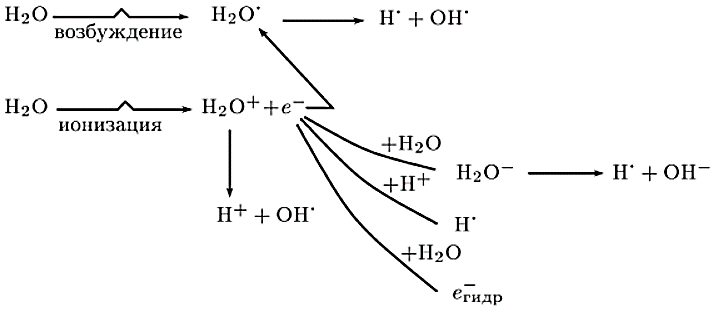
\includegraphics[width=\textwidth]{radiolysisOfWater.png}
    \caption{Схема образования первичных продуктов радиолиза воды}
    \label{radiolysisOfWater}
\end{figure}
Первичные продукты радиолиза воды – радикалы $H', OH'$, \ce{e^{-}_{гидр.}}, – располагаются
в пространстве достаточно близко друг от друга, образуя своеобразные скопления –
«рои» небольшого объема, средний радиус которых около 1,5 нм. Радиохимики
называют эти скопления шпурами. В среднем на шпур приходится около 6 радикалов.Именно в шпуре происходит рекомбинация радикалов с образованием молекулярных
продуктов – $Н_2$ и $Н_2О_2$.

Атаковать растворенные молекулы могут лишь те радикалы, которые не
рекомбинируют, а выходят из шпура. Эти радикалы, а также молекулярные продукты
радиолиза мы будем называть продуктами радиолиза воды. Образование их отражает
следующее суммарное уравнение:
\[ H_2O \rightarrow H' + OH^{+} + \ce{e^{-}_{гидр.}} + H_2 + H_2O_2 + H_3O^{+},\]
где $H_3O^{+}$ – принятая форма записи иона $H^{+}$, уравновешивающего
отрицательный заряд гидратированного электрона.

\begin{wraptable}{R}{.35\textwidth}
    \caption{Радиационно-химический выход продуктов радиолиза воды}\label{radioOutput}
    \begin{tabular}{|C{2.7 cm}|C{2.5 cm}|} \hline
    Продукты радиолиза воды & Значение G \\ \hline
    \ce{e^{-}_{гидр.}} & 2,6 \\  \hline
    $H'$ & 0,6 \\  \hline
    $OH'$ & 2,6 \\  \hline
    $H_2O_2$ & 0,75 \\  \hline
    $H_2$ & 0,45 \\  \hline
    \end{tabular}
\end{wraptable}
В таблице \ref{radioOutput} приведены радиационно-химические выходы $G$ продуктов радиолиза воды.

Оказалось, что при нейтральном значении рН на каждые 100 эВ поглощенной энергии излучения в наибольшем количестве образуются гидратированные электроны и радикалы $OH'$. 

Для исследования механизмов взаимодействия продуктов радиолиза воды и растворенных макромолекул необходимо располагать надежными методами идентификации продуктов радиолиза и уметь определять их количество. Количество молекулярных продуктов – $H_2$ и $H_2O_2$ – оценивают стандартными методами химического анализа. Наличие гидратированного электрона можно зарегистрировать по характерному спектру оптического поглощения. Спектр поглощения радикала $OH'$ регистрируют в области ниже 300 нм. В сочетании перечисленные методы позволяют исследовать типы реакций, происходящих при взаимодействии продуктов радиолиза воды с органическими молекулами. 

% \textbf{Основная литература:}
% \begin{enumerate}
%     \item 
% \end{enumerate}
\end{document}